\chapter{Learning Continuous-Action Diffusion Policies}
\label{ch:diffusion-policies}

\aigen{\emph{This chapter is based on joint work with Zhihan Huang and Yuting Wei \citep{tan2026learning}: Kevin Tan, Zhihan Huang, and Yuting Wei, ``Learning Diffusion Policies with Sublinear Regret,'' working paper, 2026.}}

\todoresolve{CHAPTER 5 IS BASED ON YOUR WORKING PAPER WITH ZHIHAN HUANG AND YUTING WEI (LEARNING DIFFUSION POLICIES WITH SUBLINEAR REGRET). AI-GENERATED CHAPTER HEADER AND ALGORITHM-NAME REPLACEMENTS (ALGORITHM 1, ALGORITHM 2, ALGORITHM 3 INSTEAD OF DIPO-BC / DIPO-FQI) ARE IN GREEN.}

\section{Introduction}

Originally introduced as a novel approach to policy modeling in robotics \citep{chi2023diffusionpolicy}, diffusion policies have rapidly become a powerful and influential framework in reinforcement learning (RL) \citep{black2023training,ren2024diffusionpolicypolicyoptimization, yang2023policyrepresentationdiffusionprobability, hansenestruch2023idqlimplicitqlearningactorcritic, wang2023diffusionpoliciesexpressivepolicy, psenka2024learningdiffusionmodelpolicy, li2024learningmultimodalbehaviorsscratch}, attracting substantial attention due to their ability to model complex, multimodal and stochastic decision rules \citep{li2024learningmultimodalbehaviorsscratch, ren2024diffusionpolicypolicyoptimization}. 
This surge of interest has led to the development of a diverse set of methods for learning diffusion-based policies within both online and offline RL. 
In online RL, proposed approaches include policy gradient-based optimization \citep{ren2024diffusionpolicypolicyoptimization}, behavior cloning \citep{chi2023diffusionpolicy}, critic-induced greedy sampling \citep{yang2023policyrepresentationdiffusionprobability, li2024learningmultimodalbehaviorsscratch}, and score-function alignment with critic gradients \citep{psenka2024learningdiffusionmodelpolicy}. 
Within offline RL, \citet{wang2023diffusionpoliciesexpressivepolicy} proposes a score-matching objective on the behavior policy, augmented with a Q-value maximization term incorporated directly into the training loss. 


% This has precipitated the development of a zoo of different methods available for learning diffusion policies within the literature. Within prior work, numerous approaches exist for online RL -- including employing policy gradient updates \citep{ren2024diffusionpolicypolicyoptimization}, behavior cloning \citep{chi2023diffusionpolicy} a greedy policy induced by the critic \citep{yang2023policyrepresentationdiffusionprobability, li2024learningmultimodalbehaviorsscratch}, or even matching the score estimate to the critic action gradient \citep{psenka2024learningdiffusionmodelpolicy}. In the context of offline RL, \citet{wang2023diffusionpoliciesexpressivepolicy} perform score-matching on the behavior policy while adding a term maximizing Q-values into the diffusion model loss. 

Recent work has begun to clarify the theoretical properties of diffusion policies. For instance, \citet{psenka2024learningdiffusionmodelpolicy} show that the policy gradient theorem \citep{sutton1999policygradient} applies to diffusion model sampling, while \citet{yang2023policyrepresentationdiffusionprobability} establish a PAC guarantee for diffusion behavior cloning given an accurate score estimate. \citet{kveton2024onlineposterior} study diffusion models as priors over unknown reward parameters in contextual bandits. More recently, \citet{vu2026expressivity} quantify the trade-off between diffusion-policy expressivity and statistical complexity. Their empirical objective requires evaluating candidate policies on counterfactual trajectories generated from the same sampled initial states and noise sequences, which operationally can be realized by a simulator with reusable randomness. This leaves open an online regret guarantee that accounts for exploration and adaptive sampling. We ask:
\begin{center}
    \textit{Can one obtain provable sublinear regret for diffusion policies at all, despite their iterative denoising structure, stochastic samplers, and intractable policy densities?}
\end{center}
Specifically, we consider two representative classes of algorithms for online RL with diffusion policies. The first performs policy optimization over diffusion policies using the policy gradient theorem \citep{ren2024diffusionpolicypolicyoptimization}. The key difficulty is that diffusion policies are implicit: we can sample from them, but the terminal action density is generally intractable. For vanilla PG, an unbiased policy-score estimate is sufficient. For NPG, the issue is more delicate, since the update is a least-squares problem in policy-score features, whose covariance is not generally recovered from the sampled denoising-path score.

The second class learns a critic and behavior-clones its greedy policy \citep{chi2023diffusionpolicy, yang2023policyrepresentationdiffusionprobability, li2024learningmultimodalbehaviorsscratch}. This reduces policy learning to supervised action prediction \citep{foster2024behaviorcloningneedunderstanding}, but introduces a different diffusion-specific issue: the diffusion sampler must match a critic-induced greedy policy, which is deterministic conditional on the state. 


We show that these diffusion-specific obstacles do not preclude sublinear regret. Our analysis establishes that, under the stated regularity conditions, one does not pay an additional statistical regret-order penalty merely because the policy is implemented through diffusion sampling. Approximation and sampling errors are retained explicitly. For policy
optimization, we recover usable policy-score features from the sampler. Vanilla PG uses an unbiased denoising-path score estimate for DDPM \citep{psenka2024learningdiffusionmodelpolicy} or the exact policy score for DDIM, while our NPG analysis uses the exact DDIM score features (Lemma \ref{lem:feature-concentration-ddim}). For NPG, we compare with a policy of finite initial KL divergence and retain its gap to the optimal value, since a deterministic optimal policy may have infinite KL divergence relative to the initial policy. 
We also give a gradient-domination lemma under coverage, compatible advantage approximation, and conditioning of the positive Fisher spectrum \citep{agarwal2021policygradient, mei2022globalconvergenceratessoftmax}. It allows redundant parameters through the Fisher pseudoinverse and retains the error in representing the advantage by policy-score features. For behavior cloning, existing diffusion model guarantees do not directly apply because the greedy
target is deterministic. We handle this with a Wasserstein smoothing argument and track the initialization, sampling, and
score-matching errors over $K$ denoising steps.

The expressivity of the actor matters even before optimization: fitting a single Gaussian to two separated rewarding modes can put most of its mass between them. We also exhibit a family with exponentially many combinations of modes that a diffusion actor represents with $O(d)$ denoising units, while a flat Gaussian mixture needs exponentially many components. When the mode probabilities are unknown, the structured actor can be learned from polynomially many demonstrations (Appendix~\ref{app:representation}).
We summarize the resulting guarantees as follows.


\textbf{Policy optimization.}
Under reset or mixing access and the stated coverage and regularity conditions, vanilla PG achieves $O(T^{3/4})$ expected regret up to approximation and comparator errors. Its mixing guarantee requires a policy-independent stationary state law, and its density-ratio factor can be exponential in the effective horizon \citep{agarwal2021policygradient}. DDIM NPG also achieves $O(T^{3/4})$ regret with high probability, up to approximation and comparator errors, while replacing this
density-ratio dependence by a transfer condition on the compatible approximation \citep{kakade2001npg, song2022denoisingdiffusionimplicitmodels}. For NPG, the stationary state law may depend on the policy. Hybrid NPG retains the $O(T^{3/4})$ statistical exponent when logged trajectories from a known behavior policy provide importance-weighted Monte Carlo labels with bounded score-weighted second moments. The construction preserves the offline feature distribution, so offline features can supply directions missing from online samples, without restarting at their stored states or fitting a critic.

\textbf{Behavior cloning.}
In finite-horizon RL, critic cloning \citep{li2024learningmultimodalbehaviorsscratch, yang2023policyrepresentationdiffusionprobability} achieves a $\widetilde O(\sqrt T)$ regret bound for controlled critic complexity,
up to cumulative score-matching and sampler errors, by decomposing the regret into critic-estimation and behavior-cloning errors. As in \citet{song2023hybrid}, offline data with sufficient Bellman-error coverage
can remove the need for optimism.
The distinction between these routes also concerns exploration. Our policy-gradient guarantees assume that the available trajectories cover the relevant state-action directions. An expressive actor alone does not ensure that it visits states needed to discover a good policy. Critic cloning instead uses optimism to choose informative actions online, or uses offline Bellman-error coverage in the hybrid case. The price is that the actor must track the changing critic well enough for its accumulated cloning error to remain small.

% \paragraph{What is new?}
% We ask whether diffusion policies can enjoy sublinear regret despite being implemented by iterative denoising samplers with generally intractable terminal densities. This is not automatic. For
% policy optimization, even writing down the policy score is delicate. The vanilla PG guarantee relies on unbiased DDPM and DDIM score estimates as noted in \cite{psenka2024learningdiffusionmodelpolicy}, as well as a novel gradient-domination lemma for Lipschitz policy classes with positive definite information matrix \citep{agarwal2021policygradient, mei2022globalconvergenceratessoftmax}, which may be of independent interest.
% The DDIM NPG guarantee relies on a result in Lemma \ref{lem:feature-concentration-ddim} that the DDIM policy score is a reparameterization of the initial noise draw within the sampling procedure.
% This yields another insight into diffusion policy gradients, that they may not track the true “denoising score function”, but instead optimize over a universal Lipschitz policy class.

% With behavior cloning, existing diffusion model guarantees do not apply as we behavior-clone a deterministic greedy policy. This requires a Wasserstein smoothing argument in tracking the diffusion sampling procedure over $K$ steps to investigate how sampling error and score matching error affect regret. 
% Our analysis establishes that when one chooses an expressive diffusion policy class, one does not pay an additional regret-order penalty merely because the policy is implemented through diffusion sampling. 

% \textbf{Policy optimization.}
% We analyze diffusion policy optimization in infinite-horizon discounted RL under coverage assumptions. These encompass the reset \citep{kakade2001npg, kakade2002approxoptimalrl, bagnell2003psdp, agarwal2021policygradient, zhou2023offlinedataenhancedonpolicy}, mixing \citep{gaur2023globalconvergencenaturalactorcritic, wu2022finitetimeanalysistimescale, xu2021improvingsamplecomplexitybounds, kausik2023mixtures}, or offline-to-online \citep{song2023hybrid, amortila2024harnessing, nakamoto2023calql, kausik2024leveragingofflinedatalinear} settings. Vanilla PG achieves $O(T^{3/4})$ regret using a pathwise DDPM/DDIM score identity, but pays a density-ratio term that can be exponential in the effective horizon \citep{agarwal2021policygradient}. DDIM NPG also achieves $O(T^{3/4})$ regret while removing this density-ratio dependence, but relies on reparameterizing the DDIM policy score through the initial Gaussian noise \citep{kakade2001npg, song2022denoisingdiffusionimplicitmodels}.  

% \textbf{Behavior cloning.} 
%  We analyze this within finite horizon RL by having a diffusion policy imitate the greedy policy induced by the current critic as in \citet{li2024learningmultimodalbehaviorsscratch, yang2023policyrepresentationdiffusionprobability}. Decomposing the regret into the errors from behavior cloning and critic estimation allows us to achieve a $O(\sqrt{T})$ regret bound -- as long as one can accurately estimate the score. As in \citet{song2023hybrid}, we further show that one can omit the use of optimism given access to an offline dataset with sufficient coverage.

 

% Specifically, we consider two representative classes of algorithms for online RL with diffusion policies. The first class performs policy optimization over diffusion policies using the policy gradient theorem \citep{ren2024diffusionpolicypolicyoptimization}. This setting presents a key challenge: although we can sample from the diffusion policy, its explicit density is intractable.
% To overcome this, \citet{psenka2024learningdiffusionmodelpolicy} demonstrate that the trajectory log-likelihood can serve as a surrogate for the log-policy term within the policy gradient estimate, yielding strong empirical performance \citep{ren2024diffusionpolicypolicyoptimization}. 

% The second class employs behavior cloning \citep{chi2023diffusionpolicy} to imitate the greedy policy from a Q-function estimate \citep{yang2023policyrepresentationdiffusionprobability, li2024learningmultimodalbehaviorsscratch}. 
% Behavior cloning reduces the problem of imitation learning to a supervised learning problem of predicting a policy's actions given states \citep{foster2024behaviorcloningneedunderstanding}.
% This is naturally applicable to the class of diffusion policies, where one can seek to match the target distribution of an expert policy conditional on the state \citep{chi2023diffusionpolicy}.
% This can be interpreted as Q-learning with an exploration policy parameterized by a diffusion model.


% We summarize our main results and contributions as follows. 

% \begin{itemize}
% \item



% \textbf{Policy optimization.} We analyze diffusion policy policy optimization in the context of infinite-horizon discounted RL under a broad array of coverage assumptions encompassing the reset distribution setting Options include the \emph{reset distribution} setting \citep{kakade2001npg, kakade2002approxoptimalrl, bagnell2003psdp, agarwal2021policygradient, zhou2023offlinedataenhancedonpolicy}, where the agent can reset the environment to an initial state $s_0 \sim \nu$. Another is the \emph{strong mixing} setting \citep{gaur2023globalconvergencenaturalactorcritic, wu2022finitetimeanalysistimescale, xu2021improvingsamplecomplexitybounds}. Yet another is having access to an \emph{offline dataset} $\gD_{\off}$ \citep{song2023hybrid, amortila2024harnessing, nakamoto2023calql}.

% We obtain a $O(T^{3/4})$ regret bound for the vanilla policy gradient method under coverage assumptions. 
% This relies on a novel gradient domination lemma \citep{agarwal2021policygradient, mei2022globalconvergenceratessoftmax} for Lipschitz policy classes with positive definite information matrix, which may be of independent interest. 

% The result depends on the maximum density ratio of the optimal policy's state occupancy and the reset distribution, which can be exponential in the effective horizon \citep{agarwal2021policygradient}. Natural policy gradient \citep{kakade2001npg} updates can yield stronger provable guarantees independent of the above ratio \citep{agarwal2021policygradient}. However, having access to only the trajectory log-density leads to inconsistent NPG update estimates. We bypass this when a deterministic ODE sampler \citep{song2022denoisingdiffusionimplicitmodels} is used, with $O(T^{3/4})$ regret independent of the density ratio. 
% Finally, we show NPG does not require reset distribution coverage when an offline dataset with sufficient coverage is available. 

% \item 




% \textbf{Novelty and technical challenges.} We show that diffusion policies do indeed recover familiar rates in $T$ within the RL theory literature. But these rates do not carry over for free. For diffusion policies, even writing down the policy score is delicate. The vanilla PG guarantee relies on unbiased DDPM and DDIM score estimates as noted in \cite{psenka2024learningdiffusionmodelpolicy}, as well as a novel gradient-domination lemma for Lipschitz policy classes with positive definite information matrix \citep{agarwal2021policygradient, mei2022globalconvergenceratessoftmax}, which may be of independent interest.
% The DDIM NPG guarantee relies on a result in Lemma \ref{lem:feature-concentration-ddim} that the DDIM policy score is a reparameterization of the initial noise draw within the sampling procedure. 
% This yields another insight into the diffusion policy gradient algorithm, that DPPO may not track the true “denoising score function”, but instead optimizes over a universal Lipschitz policy class.

% With behavior cloning, existing diffusion models guarantees do not immediately apply as we behavior-clone a deterministic greedy policy, requiring a Wasserstein smoothing argument as well as tracking the diffusion sampling procedure over $K$ steps in investigating how sampling error and score matching error affect regret. 
% Our analysis establishes that when one chooses an expressive diffusion policy class, one does not pay an additional regret-order penalty merely because the policy is implemented through diffusion sampling. 

Finally, our experiments compare practical versions of these algorithmic families and show that several tested diffusion-policy methods exhibit sublinear empirical regret across standard Gym and Robomimic benchmarks.


\begin{table}
\centering
\small
\setlength{\tabcolsep}{3pt}
\begin{tabular}{@{}>{\raggedright\arraybackslash}p{0.18\linewidth}>{\raggedright\arraybackslash}p{0.34\linewidth}>{\raggedright\arraybackslash}p{0.43\linewidth}@{}}
\toprule
Method & Sampling access & Regret \\
\midrule
Vanilla PG & Resets or fixed-state mixing & $O(T^{3/4})$ + comparison-policy and compatible-approximation errors \\
DDIM NPG & Resets, mixing, or hybrid data & $O(T^{3/4})$ + comparison-policy and advantage-transfer errors \\
Critic cloning & Online interaction, optionally with offline data & $\widetilde O(\sqrt T)$ + cumulative actor error \\
\bottomrule
\end{tabular}
\vspace{1ex}
\caption{Summary of results for fixed regularity constants. PG bounds include approximation and comparator errors. The vanilla PG bound is in expectation, while NPG and critic cloning hold with high probability. The critic contribution is $O(H^2\sqrt{\beta T\mathsf{SEC}(\gF,\Pi,T)})$, with $\beta$ defined in Theorem~\ref{thm:dipo-bc-regret}. The table suppresses these exploration and critic-class factors.}
\label{tab:cost-map}

\end{table}


\section{Setup and Background}

\paragraph{RL Notation.} We examine two standard RL models. An infinite-horizon discounted MDP is a tuple $(\gS, \gA, \gamma, \prob, r)$ with $r \in [0,1]$ and $\gamma \in (0,1)$. We take $\gA \subseteq \R^{d_A}$, with $\|a\|\leq R_A$ in the behavior-cloning analysis. Policy gradients use actions in $\R^{d_A}$ or a fixed invertible output transformation into the action domain. 
From a starting state distribution $\rho$ and policy $\pi$, write
$$\textstyle{V^\pi(s) = \E_{\pi} \left[\sum_{h=0}^\infty \gamma^h r(s_h,a_h) | s_0 = s\right]}, \enspace {Q^\pi(s,a) = \E_{\pi} \left[\sum_{h=0}^\infty \gamma^h r(s_h,a_h) | s_0 = s, a_0 = a\right].}$$
The advantage function is \mbox{$A^\pi(s,a) = Q^\pi(s,a) - V^\pi(s)$.} Write $V^\pi(\rho) = \E_{s \sim \rho}[V^\pi(s)]$. The optimal policy $\pi^*$ maximizes $V^\pi$. We write $V^* = V^{\pi^*}$ and do the same for $Q^*$ \& $A^*$.


In the finite-horizon setting, an MDP is a tuple $(\mathcal{S},\mathcal{A}, H,\{\prob_h\}_{h=1}^{H} ,\{r_h\}_{h=1}^{H})$, with time-dependent
$$\textstyle{V_h^{\pi}(s) = \mathbb{E}\left[\sum_{h'=h}^{H}r_{h'}(s_{h'},a_{h'})|s_h = s\right], \enspace Q_h^{\pi}(s,a) = \mathbb{E}\left[\sum_{h'=h}^{H}r_{h'}(s_{h'},a_{h'})|s_h = s,a_h=a\right]}.$$
$Q^*$ is the unique solution to the Bellman equation $Q_h^* = \gT_h Q_{h+1}^*$:
$$
    \mathcal{T}_{h}Q_{h+1}(s,a) = r_h(s,a) + \mathbb{E}_{s'}[\max_{a'\in\mathcal{A}}Q_{h+1}(s',a')],
    \mathcal{T}^\pi_{h}Q_{h+1}(s,a) = r_h(s,a) + \mathbb{E}_{s'}Q_{h+1}(s',\pi_{h+1}).
$$
In both settings, observed rewards lie in $[0,1]$ and have conditional mean $r(s,a)$ or $r_h(s,a)$ given the current state, action, and past. At round $t=1,...,T$ the agent deploys a policy $\pi^{(t)}$ parameterized by some $\theta^{(t)} \in \Theta \subseteq \R^p$, and incurs regret 
$\textstyle{\text{Reg}(T) := \sum_{t=1}^T \left(V^*(\rho) - V^{(t)}(\rho)\right)}$ where $V^{(t)} := V^{\pi^{(t)}}$.
%Another goal in this setting is to find some policy $\hat{\pi}$ such that $V^* - V^{\hat{\pi}} \leq \epsilon$ in as few steps as possible.


\paragraph{Diffusion models.}
A diffusion model samples an initial noise vector $Y_K\sim N(0,I_{d_A})$, applies $K$ denoising
steps conditional on the state $s$, and plays the terminal action $Y_0$.
Let $\epsilon_\theta(\cdot,k,s)$ be the trainable denoising field conditional on state $s$.
With $\bar{\alpha}_k \coloneqq \prod_{i=1}^k \alpha_i$, the DDIM-type \citep{song2022denoisingdiffusionimplicitmodels} and DDPM-type \citep{ho2020denoising} update rules for $k=K,...,1$ are 
\begin{align}
    Y_{k-1} &\gets \alpha_k^{-\frac{1}{2}}\big(Y_k + \eta_k^{\mathsf{ddim}} \epsilon_{\theta}(Y_k, k, s)\big) =: \Phi_k^\theta(Y_k). \label{eq:DDIM}\\
    Y_{k-1} &\gets \alpha_k^{-\frac{1}{2}}\big(Y_k + \eta_k^{\mathsf{ddpm}} \epsilon_{\theta}(Y_k, k, s) + \sigma_k^{\mathsf{ddpm}} Z_k\big)
    =: \Psi_k^\theta(Y_k, Z_k). \label{eq:DDPM}
\end{align}
Here $Z_k$ are independent standard Gaussian vectors, independent of $Y_K$. We write $\Phi_{k_2:k_1}(Y_{k_2}) = (\Phi_{k_1+1} \circ ... \circ \Phi_{k_2})(Y_{k_2})$ for the composition of DDIM updates from times $k_1 \leq k_2$, and $\Psi^{(t)}, \Phi^{(t)}$ as shorthand for $\Psi^{\theta^{(t)}}, \Phi^{\theta^{(t)}}$ and omit the dependence on $s$. Here $\eta_k^{\mathsf{ddim}}$, $\eta_k^{\mathsf{ddpm}}$ and $\sigma_k^{\mathsf{ddpm}}$ are design parameters that admit multiple alternatives. For policy-gradient sampling, we choose positive, parameter-independent DDPM transition variances at every step, including the final transition. Section~\ref{sec:behavior-clone} specifies the different coefficients and stopping rule used for behavior cloning. A key technical issue here is that the distribution of $Y_0$ is implicit: we can sample actions, but the terminal density
$\pi_\theta(a\mid s)$ and its score are not generally available.


% \paragraph{Diffusion models.}
% Diffusion models encompass two Markov processes, described in \citep{ho2020denoising,sohl2015deep}. The forward process is given by a sequence of $d_A$-dimensional random vectors $X_1 \to ... X_K$: $X_0 \sim p_{\text{data}}, X_k = \sqrt{\alpha_k}X_{k-1} + \sqrt{1-\alpha_k} W_k$,
% where $\alpha_k \in (0,1)$ can be regarded as the learning rate and $W_k \stackrel{\text{i.i.d.}}{\sim} \gN(0,\mathbf{I}_{d_A})$. The reverse process seeks to construct a series of random vectors $(Y_k)_{k=1}^K$ such that $X_k \stackrel{d}{\approx} Y_{K-k}$. 
% From a differential equation perspective, the forward process is the discretization of the SDE $\d X_t = -b(t) X_t \d t + \sqrt{2b(t)} \d B_t$ for some function $b(t)$.
% To reverse this process, one can either use the probability flow ODE \citep{song2020score}, or construct a ``reverse-time'' SDE \citep{anderson1982reverse}:
% \begin{align*}
%     &\d Y_t = \left(Y_t + \nabla \log p_{T-t}(Y_t)\right)b(T-t) \,\d t,\\
%     &\d Y_t = \left(Y_t + 2 \nabla \log p_{T-t}(Y_t)\right)b(T-t)\, \d t + \sqrt{2b(T-t)} \, \d W_t.
% \end{align*}
% Both of these differential equations enjoy matching marginal distributions with the forward SDE, i.e., $X_t \overset{\d}{=} Y_{K-t}$ as long as we generate $Y_0 \overset{\d}{=} X_K$. The Stein score function $\nabla \log p_{T-t}(\cdot)$ in the backward process is unknown in general. 
% Denoising score matching \citep{vincent2011connection} is commonly used to learn to inject noise into the forward process:
% $\epsilon(\cdot,t) = \argmin_{\epsilon}\E_{X_0,X_t}\left[\|\epsilon(X_t,t) - (X_t - X_0)\|_2^2\right]$,
% From this quantity, one can apply Tweedie's formula \citep{efron2011tweedie} to recover $\nabla \log p_{T-t}(\cdot)$. 
% % \zh{add introduction of using score matching to learn $\epsilon_{\theta}(x,k)$} 

% Applying suitable discretization schemes leads to widely-used DDIM-type \citep{song2022denoisingdiffusionimplicitmodels} and DDPM-type samplers \citep{ho2020denoisingdiffusionprobabilisticmodels}.
% Suppose we have access to $\epsilon_\theta(\cdot,t,s)$ as an estimator of $\epsilon(\cdot, t)$ conditional on the state $s$ in MDP.
% With $\bar{\alpha}_k \coloneqq \prod_{i=1}^k \alpha_i$, the update rules for $k=K,...,1$ are 
% \begin{align}
%     Y_{k-1} &\gets \alpha_k^{-\frac{1}{2}}\big(Y_k + \eta_k^{\mathsf{ddim}} \epsilon_{\theta}(Y_k, k, s)\big) =: \Phi_k^\theta(Y_k). \label{eq:DDIM}\\
%     Y_{k-1} &\gets \alpha_k^{-\frac{1}{2}}\big(Y_k + \eta_k^{\mathsf{ddpm}} \epsilon_{\theta}(Y_k, k, s) + \sigma_k^{\mathsf{ddpm}} Z_k\big)
%     =: \Psi_k^\theta(Y_k, Z_k). \label{eq:DDPM}
% \end{align}
% We write $\Psi_{k_2:k_1}(Y_{k_2}) = \Psi_{k_1+1} \circ ... \circ \Psi_{k_2}(Y_{k_2})$ for the composition of DDIM updates from times $k_1 \leq k_2$, and $\Psi^{(t)}, \Phi^{(t)}$ as shorthand for $\Psi^{\theta^{(t)}}, \Phi^{\theta^{(t)}}$ and omit the dependence on $s$. Here $\eta_k^{\mathsf{ddim}}$, $\eta_k^{\mathsf{ddpm}}$ and $\sigma_k^{\mathsf{ddpm}}$ are design parameters that admit multiple alternatives, which are asymptotically equivalent with slightly different finite iteration performance. In this manuscript, we adopt the parameter choice in \citet{liang2025low}.


\paragraph{Expressivity.} A policy may need to retain several good actions at a state, for example when cloning demonstrations with distinct modes. Fitting one Gaussian can place mass between these actions, where reward is low. In Appendix~\ref{app:representation}, we give a two-mode example in which the population maximum-likelihood Gaussian loses almost all reward. Directly optimizing reward can instead choose one good mode, so the example concerns the distribution-matching objective used in cloning.

\begin{exmp}[Representing and learning combinations of modes]
A more pronounced difference appears when each of $d$ action coordinates has two independently chosen modes. There are $2^d$ joint combinations, but a denoiser can generate them coordinate by coordinate. Proposition~\ref{prop:flat-gmm-separation} realizes a fixed-accuracy approximation with $O(d)$ tanh units, whereas any flat Gaussian mixture attaining total variation error $0.01$ needs at least $0.79\cdot2^d$ components. If the coordinate probabilities are unknown and lie in $[1/4,3/4]$, Proposition~\ref{prop:learned-product-mixture} learns an $O(d)$-unit actor from $O(d\log(d/\delta)/\varepsilon^2)$ independent demonstrations with total variation error at most $\varepsilon$, with probability at least $1-\delta$. A flat mixture still needs exponentially many components at fixed accuracy. Thus the product structure permits learning a compact actor from polynomially many demonstrations. The comparison uses the same demonstrations and distribution-matching objective for both families.
\end{exmp}

\section{Diffusion Policies with Policy Optimization}
\label{sec:policy-opt}

Policy gradient methods seek to solve the optimization problem $\max_{\theta \in \Theta} V^{\pi_\theta}(\rho)$, where $\{\pi_\theta : \theta \in \Theta\}$ is a policy class parametrized by $\theta \in \Theta$, and $\rho \in \Delta(\gS)$. 
At round $t$, given some $\theta^{(t)} \in \Theta$, one rolls out a trajectory under $\pi^{(t)} = \pi_{\theta^{(t)}}$, and uses the observed state $s^{(t)}$, action $a^{(t)}$, and rewards to estimate an update direction for $\theta^{(t)}$. One candidate utilizes the policy gradient theorem \citep{sutton1999policygradient}:
\begin{equation}
    (1-\gamma)\nabla_\theta V^{\pi_\theta}(\rho) = \E_{d_\rho^{\pi_\theta}}\left[A^{\pi_\theta}(s,a) \nabla_\theta \log \pi_{\theta}(a|s)\right]
\label{eq:policy-gradient-thm}
\end{equation}
where we substitute $A$ for $Q$ as $\int_a\nabla_\theta\pi_\theta(a|s) \d a = 0$. This relies on the discounted occupancy:
$$d_\nu^\pi(ds,da):=(1-\gamma)\sum_{h\geq0}\gamma^h
\mathbb{P}_\nu^\pi(S_h\in ds,A_h\in da),\qquad S_0\sim\nu,\quad A_h\sim\pi(\cdot\mid S_h).$$
Here $\nu$ is the initial-state law. We write $d_\nu^\pi(s,a)$ for the density of this state--action measure when it exists.

\paragraph{Coverage.} To control the error under $\rho$, we have to make a coverage assumption. Options include the \emph{reset distribution} setting \citep{kakade2001npg, kakade2002approxoptimalrl, bagnell2003psdp, agarwal2021policygradient, zhou2023offlinedataenhancedonpolicy}, where the agent can reset the environment to an initial state $s_0 \sim \nu$. Another is the \emph{strong mixing} setting \citep{gaur2023globalconvergencenaturalactorcritic, wu2022finitetimeanalysistimescale, xu2021improvingsamplecomplexitybounds}. Yet another is having access to an \emph{offline dataset} $\gD_{\off}$ \citep{song2023hybrid, amortila2024harnessing, nakamoto2023calql}.

\begin{aspt}[Sampling access]\label{aspt:coverage}
Policies are fixed within each batch. We have one of the following forms of access:
\begin{enumerate}[label=(\alph*),leftmargin=*,itemsep=2pt,topsep=3pt]
\item independent trajectories initialized from a fixed state law $\nu$;
\item a continuing trajectory whose policy-induced state kernel $K_\theta$ has stationary law $m_\theta$ and satisfies $\sup_{\theta,s}\operatorname{TV}(K_\theta^h(s,\cdot),m_\theta)\leq c_{\rm mix}\kappa^h$ for $c_{\rm mix}\geq1$ and $0<\kappa<1$. Vanilla PG uses a common stationary state law $m_\theta=m$, while NPG permits dependence on $\theta$;
\item ordinary online interaction initialized from $\rho$, together with independent logged behavior trajectories whose initial state--action law is $\mu$. The known behavior policy can be evaluated and sampled at stored states.
\end{enumerate}
\end{aspt}
Otherwise, we would have to consider strategic exploration, for which incorporating policy optimization is currently a nascent area of research.\footnote{Most papers that consider strategic exploration in policy optimization employ the softmax mirror descent update \citep{zhong2023theoreticalanalysisoptimisticproximal, liu2023optimisticnaturalpolicygradient, tan2025actorcriticsachieveoptimalsample, sherman2024rateoptimalpolicyoptimizationlinear, cassel2024warmupfreepolicyoptimization}. While \cite{lin2026optimistic} considers parameterized updates, they essentially clone the softmax update using a KL projection.} We will address strategic exploration in the following section on behavior cloning.

Mixing replaces resets by a burn-in period followed by complete return samples. Hybrid NPG combines online samples with logged trajectories. It does not restart the environment at recorded states. Its importance-weighted labels require absolute continuity and finite score-weighted return moments, stated in Appendix~\ref{app:hybrid-reset-dist}. Reserved independent trajectory blocks make these labels valid for adaptively chosen policies. The online part may also use the continuing sampler under the mixing condition in (b).

Write $q_\theta$ for the state--action law used to fit an update. It is $d_\nu^{\pi_\theta}$ under resets, $m_\theta\pi_\theta$ under mixing, and $(d_\rho^{\pi_\theta}+\mu)/2$ for hybrid NPG, replacing the online component by $m_\theta\pi_\theta$ for a continuing hybrid trajectory. For vanilla PG the first two laws both have the form $d_\nu^{\pi_\theta}$, with $\nu=m$ in the mixing case. For any state--action law, a subscript $S$ denotes its state marginal. Let $\bphi^\theta(s,a)=\nabla_\theta\log\pi_\theta(a\mid s)$ and $\bLambda^\theta=\E_{q_\theta}[\bphi^\theta\bphi^{\theta\top}]$ be the policy-score feature and its covariance. The next condition requires coverage only in directions these features can identify.

A continuous action density assigns zero probability to any fixed action. Consequently, if an optimal policy always chooses one action, its state--action law is not dominated by the sampled policy law, and its KL divergence from that policy is infinite. These are separate obstacles for the density-ratio argument used by vanilla PG and the KL argument used by NPG.

We therefore compare with a fixed stochastic policy, denoted $\pi_{\rm cmp}$, and retain its value gap $V^*(\rho)-V^{\pi_{\rm cmp}}(\rho)$ in regret against the optimum. This policy need not belong to the learned class. We write $d_\rho^{\pi_{\rm cmp}}$ for its discounted occupancy and keep it fixed during learning. Example~\ref{ex:small-ball-comparator} constructs such a policy by restricting the initial actor to actions near an optimum, and shows when its value gap can be $O(T^{-1/2})$.

For now, we make an assumption that the error under $\rho$ can be related to the error under $q_\theta$ with the following concentrability assumption:
\begin{aspt}[Concentrability and score covariance]\label{aspt:npg-concentrability}
Assume $C:=\sup_\theta\|d_\rho^{\pi_{\rm cmp}}/d_\nu^{\pi_\theta}\|_\infty<\infty$ for vanilla PG, and $\lambda:=\inf_\theta\lambda_{\min}^+(\bLambda^\theta)>0$ for both algorithms, where $\lambda_{\min}^+$ denotes the smallest positive eigenvalue and the infimum runs over the update region.
\end{aspt}
The density ratio is analogous to single-policy concentrability \citep{xie2022policy}. The score covariance is the Fisher information under on-policy action sampling. Its positive spectrum controls identifiable score directions and allows redundant parameters, including under the hybrid mixture law. Under the reset law we also write this lower bound as $\lambda_{\min}^+(\bLambda_\nu)$. We use $q^{(t)}=q_{\theta^{(t)}}$, and $d^{(t)}=d_\nu^{\pi^{(t)}}$ when the sampling law has that form.

% \yuting{move Assumption 4 to this section}

% \kevin{We have to make an assumption on coverage, because the policy gradient literature on strategic exploration is still nascent. optimistic npg, optimistic actor critic exist, but are quite limited.}

% \kevin{Vanilla PG can only handle reset + fixed mixing. NPG+DDIM can handle reset, policy dependent mixing, and offline data. NPG+DDPM is screwed unless log-concave. }




\paragraph{Policy scores.}
The gradient in Equation~(\ref{eq:policy-gradient-thm}) uses the parameter score $\nabla_\theta\log\pi_\theta(a\mid s)$. The denoising field $\epsilon_\theta$ is a different object: even if it initially represents a spatial log-density gradient, a reward update need not preserve that property. Appendix~\ref{app:nonconservative-score} gives a one-step example in which a reward-improving update breaks this property while leaving the sampling map invertible and the policy differentiable.



We therefore compute the parameter score of the policy induced by the denoising map. Write $a_K,\ldots,a_0$ for a sampled path, with only $a_0$ played in the environment. However, one runs into a complication when trying to apply policy gradient updates with the DDPM sampler. As \citet{psenka2024learningdiffusionmodelpolicy} notes, evaluating the policy density $\pi_\theta(a_{0}|s)$ is intractable, involving a high-dimensional integral over the space of possible paths. Still, the policy gradient can be estimated using the transition densities along the sampled path. In Appendix B.1, \citet{psenka2024learningdiffusionmodelpolicy} show the policy gradient is equal to

\begin{equation}
(1-\gamma)\nabla_\theta V^{\pi_\theta}(\nu)
=\E\left[A^{\pi_\theta}(s,a_0)\sum_{k=1}^{K}
\nabla_\theta\log\pi_\theta(a_{k-1}\mid a_k,s)\right],
\label{eq:diffusion-pg-thm}
\end{equation}
where $(s,a_0)\sim d_\nu^{\pi_\theta}$ and the expectation includes its sampled
denoising path.
This makes the vanilla policy gradient update tractable for the DDPM sampler, though we will see later that this still remains an issue for second-order methods. Regarding the DDIM sampler, we will show in Lemma \ref{lem:feature-concentration-ddim} that we can indeed evaluate $\nabla_\theta \log\pi_\theta(a_0 | s)$ under sufficient assumptions.

The same environment advantage weights every denoising step in Equation~(\ref{eq:diffusion-pg-thm}), because only the terminal action affects the environment reward. Additional discounting across denoising steps, as used in \citet{ren2024diffusionpolicypolicyoptimization}, changes this estimator. We retain the environment discount $\gamma$ and analyze the undiscounted sum of denoising-path scores.




% \begin{aspt}[Lipschitz Score Functions]
%     $\epsilon_{\theta^{(t)}}(a,k,s)$ is $L_{a}$-Lipschitz in $a$, $L_s$-Lipschitz in $s$, and $L_\theta$-Lipschitz in $\theta$. Additionally, for the DDIM sampler, assume $\lVert\nabla_\theta \nabla_a \Phi_{K:0}^\theta(a_K) \rVert_2 \leq L_{\theta, a}^{(K)}$.
%     \label{aspt:lipschitz-score}
% \end{aspt}
%In other words, the reset distribution achieves sufficient coverage over the occupancy measure of the optimal policy for all features generated by the log-policy gradients of $\theta^{(t)},...,\theta^{(T)}$. 

% The next assumption is required to show the gradient domination lemma (Lemma \ref{lem:gradient-dom}) necessary for the convergence of vanilla diffusion policy gradients in Theorem \ref{thm:vanilla-pg-regret}, as well as the least squares bound in Lemma \ref{lem:least-squares-npg} necessary for the convergence of NPG with the DDIM sampler in Theorem \ref{thm:npg-regret}.
% \begin{aspt}[Unconstrained Regressions]
%     Write
%     ${\bLambda}^{\theta} = \E\left[{\bphi}^{\theta}{\bphi}^{\theta\top}\right], {\bb}^{\theta} = \E[{\bphi}^{\theta}\widehat{A}^{\theta}]$ for feature covariances and targets.
%     Let $\gG = \{\bg \in \R^p : \lVert\bg\rVert_2\leq G\}$ be so ${\bg}^\theta = ({\bLambda}^{\theta})^{-1}{\bb}^{\theta} \in \gG$ for all $\theta \in \Theta$.
%     %\left(\widehat{\bLambda}^{(t)}\right)^{-1}\widehat{\bb}^{(t)} = \argmin_{\bg \in \gG} \widehat{\gL}_A^{(t)}(g, \theta^{(t)}), \; \left({\bLambda}^{(t)}\right)^{-1}{\bb}^{(t)}= \argmin_{\bg \in \gG} {\gL}_A^{(t)}(g, \theta^{(t)})
%     \label{aspt:unconstrained-regression}
% \end{aspt}
% In the algorithm, we will work with NPG, whose gradient is estimated through a linear regression. 


\paragraph{Score estimates and regularity.}
For the sequence $(\theta^{(t)},s^{(t)},a^{(t)})_{t=1}^T$, write $\bphi^{(t)}=\bphi^{\theta^{(t)}}(s^{(t)},a^{(t)})$. The computable DDPM estimate is $\widehat\bphi^{(t)}=\sum_{k=1}^K\nabla_\theta\log\pi_\theta(a_{k-1}^{(t)}\mid a_k^{(t)},s^{(t)})$, whose conditional expectation given $(s^{(t)},a_0^{(t)})$ equals $\bphi^{(t)}$. For DDIM, the change-of-variables formula in Lemma~\ref{lem:ddpm-ddim-log-policy-densities} evaluates the endpoint score exactly, and we set $\widehat\bphi^{(t)}=\bphi^{(t)}$.

\begin{aspt}[Smoothness, moments, and invertibility]\label{aspt:ddpm-bijection}
Likelihood derivatives and expectations below may be interchanged. The following conditions hold uniformly at the iterates and along their update segments:
For DDIM, $\Phi_{K:0}^\theta$ is a smooth diffeomorphism onto a parameter-independent open action support.
Under the applicable sampling law, $\E_{q_\theta}\|\widehat\bphi\|^2\leq\beta_K^2$, including the denoising path in the DDPM expectation.
For vanilla PG, $\theta\mapsto V^{\pi_\theta}(\nu)$ is $L_V$-smooth for fixed $\nu$. For DDIM NPG, $\bphi^\theta$ is $L^{(K)}_\theta$-Lipschitz in $\theta$.
\end{aspt}
The DDIM score is evaluated on its common action support. A fixed invertible output transformation may be included in the full map.
For regression, write $\bb^\theta=\E_{q_\theta}[\bphi^\theta A^{\pi_\theta}]$ and $\gG=\{\bg\in\mathbb R^p:\|\bg\|_2\leq G\}$. We assume the minimum-norm population coefficient $\bg^\theta=(\bLambda^\theta)^\dagger\bb^\theta$ lies in $\gG$ throughout the update region. The choice $G\geq((1-\gamma)\sqrt\lambda)^{-1}$ suffices. Conditionally unbiased advantage labels give the same target $\bb^\theta$.



In line with \cite{agarwal2021policygradient}, we impose the following assumption on compatible approximation. Intuitively, the policy has to be rich enough so that the score features $\bphi^\theta$ can model the advantage function. Writing $\gL_A^d(\bg, \theta) = \E_{s,a \sim d}[(A^{\pi_\theta}(s,a) - \langle \bg, \bphi^\theta(s,a) \rangle )^2]$ for this squared residual under any state--action law $d$, assume:
\begin{aspt}[Compatible Advantage Approximation]\label{aspt:approx-realizability}
For the fixed denoising depth $K$ used by vanilla PG, assume uniformly over its
update region that
\[
\gL_A^{d_\nu^{\pi_\theta}}(\bg^\theta,\theta)
=\E_{d_\nu^{\pi_\theta}}(A^{\pi_\theta}-\langle\bg^\theta,\bphi^\theta\rangle)^2
\leq\epsilon_{\mathrm{comp}}.
\]
\end{aspt}
The score moment $\beta_K^2$ controls the noise in the gradient estimate, while compatible approximation lets us relate a small gradient to a small value gap.

\paragraph{Neural denoisers and adapters.}
Suppose $\epsilon_\theta(\cdot,k,s)$ is smooth and $L_a$-Lipschitz, with $|\eta_k^{\mathsf{ddim}}|L_a<1$ at every DDIM step. Solving for its input is then a contraction, so the step is invertible and its inverse Jacobian has norm at most $\sqrt{\alpha_k}/(1-|\eta_k^{\mathsf{ddim}}|L_a)$. On a uniformly invertible parameter region, the width-$256$ tanh MLP and smooth U-Net architectures in Appendix~\ref{app:practical-network-regularity} have finite score moments when their parameters and state conditioning are bounded. The same calculation controls averaged log-likelihood curvature if the comparison policy has a finite third moment after pulling actions back through the initial actor. The weights may be independently trained, but the Fisher and advantage-approximation conditions also depend on the MDP.

For a trainable location adapter on a frozen MLP or U-Net, we can also bound the positive Fisher spectrum in terms of the backbone's Lipschitz constant and the adapter design (Appendix~\ref{app:adapter-fisher}). The bound allows redundant parameters and applies under reset or mixing sampling, where actions follow the current policy. For the hybrid sampling law, conditioning instead follows from the mixture-covariance argument in Appendix~\ref{app:hybrid-reset-dist}.



\subsection{Monte Carlo Diffusion Vanilla Policy Gradient}
We are now in a position to analyze the vanilla policy gradient update on diffusion policies, where one uses Equation (\ref{eq:diffusion-pg-thm}) for the DDPM sampler and Equation (\ref{eq:policy-gradient-thm}) for the DDIM sampler. The algorithm we analyze is presented below in Algorithm \ref{alg:dppo-vanilla-pg}, for which we defer the proofs to Appendix \ref{app:vanilla-pg}.


\paragraph{Algorithm and score estimate.}
Algorithm~\ref{alg:dppo-vanilla-pg} is vanilla PG with the diffusion-policy score substituted for the usual log-policy score. We use $L$ policy updates and $N$ online return labels per update, for $T=LN$ labels in total. Algorithm~\ref{alg:dppo-sampler} returns a state, an accepted action and its denoising path, together with a conditionally unbiased advantage label. With reset access, it uses geometric acceptance to sample $(s,a)\sim d_\nu^{\pi_\theta}$. With mixing, it takes complete geometric returns along the continuing trajectory, after one burn-in per batch. Both implementations freeze the policy during a batch. The path is retained because the DDPM score estimate requires its transition likelihoods, whereas DDIM uses the terminal score.

% We briefly outline the algorithm design, which is largely canonical with minor tweaks. Firstly, although we wish to recover $V^*(\rho)$, we instead optimize $V^\theta(\nu)$, and transfer the error back using $\lVert d_\rho^* / \nu \rVert_\infty$. Directly optimizing $V^\theta(\rho)$ is ineffective due to nonconvexity, but we show that a notion of gradient domination \ref{lem:gradient-dom}  allows Algorithm \ref{alg:dppo-vanilla-pg} to succeed.  Secondly, we construct a sampler (Algorithm \ref{alg:dppo-sampler}) as in \citet{agarwal2021policygradient} that yields samples $s^{(t)}, a_0^{(t)} \sim d_\nu^{\pi_{\theta^{(t)}}}$, unbiased advantage estimates $\widehat{A}^{(t)}$, and auxiliary denoising actions $a_1^{(t)},...,a_K^{(t)}$.  In the fixed-mixing case in Assumption \ref{aspt:coverage}(b)(i), the sampler first runs $b$ burn-in steps under $\pi_{\theta^{(t)}}$ and then proceeds as Algorithm~\ref{alg:dppo-sampler}. This replaces exact sampling from $d_\nu^{\pi_{\theta^{(t)}}}$ by a distribution within $O(c_{\mix}\kappa^b)$ total variation distance.
% This provides nearly everything we need to estimate the policy gradient updates in Equations \ref{eq:diffusion-pg-thm} (DDPM) and \ref{eq:policy-gradient-thm} (DDIM), with only the log-policy gradient terms $\widehat{\bphi}^\theta$ (DDPM), $\bphi^\theta$ (DDIM) remaining. 

% The first diffusion-specific step is to replace the unavailable terminal score by a computable object -- a pathwise score for DDPM, and an exact change-of-variables score for DDIM. We resolve this here.
In dealing with diffusion policies, we first have to compute and bound the score features in Lemmas \ref{lem:ddpm-ddim-log-policy-densities} and \ref{lem:lipschitz-constant-policy}. Under resets or a stationary-start mixing batch, the estimators $\widehat A^{(t)}\widehat\bphi^{(t)}/(1-\gamma)$ and $\widehat A^{(t)}\bphi^{(t)}/(1-\gamma)$ are unbiased (Lemma~\ref{lem:unbiased-vanilla-pg}) for the policy gradient $\nabla_\theta V^{\pi_\theta}(\nu)$. For a finite burn-in, Theorem~\ref{thm:vanilla-pg-regret} includes the resulting coupling error. Together with the stated smoothness and second-moment conditions, this yields convergence to a stationary point: the stochastic ascent argument \citep{yuan22vanillapg} gives $\sum_{t=1}^T\E\|\nabla_\theta V^{(t)}(\nu)\|_2^2=O(\sqrt T)$. 



To relate this to regret, we prove a notion of gradient domination that bounds the suboptimality gap in terms of the policy gradient, up to approximation errors. This second step is not diffusion-specific. Once the score features are controlled, gradient domination transfers convergence to stationarity into regret. The term $\epsilon_{\rm comp}$ below is a squared advantage-regression residual. It measures how well score features fit the current advantage, whereas $V^*(\rho)-V^{\pi_{\rm cmp}}(\rho)$ measures the loss from replacing the optimal policy by the chosen stochastic comparison policy. These errors need not be related. 

\begin{lem}[Gradient Domination Lemma]\label{lem:gradient-dom}
Under Assumption~\ref{aspt:approx-realizability},
for $\rho,\nu\in\Delta(\gS)$ and $\theta$ satisfying
$C_\theta:=\|d_\rho^{\pi_{\rm cmp}}/d_\nu^{\pi_\theta}\|_\infty<\infty$,
\begin{align*}
V^*(\rho)-V^{\pi_\theta}(\rho)
\leq V^*(\rho)-V^{\pi_{\rm cmp}}(\rho)+\frac{\sqrt{C_\theta\epsilon_{\mathrm{comp}}}}{1-\gamma}+\sqrt{\frac{C_\theta}{\lambda_{\min}^+
(\bLambda^\theta_{d_\nu^{\pi_\theta}})}}
\|\nabla_\theta V^{\pi_\theta}(\nu)\|_2.
\end{align*}
\end{lem}
% \vspace{-1em}
Lemma \ref{lem:gradient-dom} bounds the suboptimality gap of $\pi_\theta$ in terms of the minimum positive eigenvalue of its score feature covariance matrix and the norm of the policy gradient, up to the approximation and comparator errors. Related results have been established for tabular MDPs, softmax MDPs, linear quadratic control, regularized linear MDPs \citep{bhandari2022globaloptimalityguaranteespolicy}, and softmax neural policies \citep{wang2019neuralpolicygradientmethods}. While used here for diffusion policies, this gradient domination lemma applies more broadly to policy classes satisfying its conditions, and so may be of independent interest.
Plugging our bounds on the rate of convergence into a stationary point into Lemma \ref{lem:gradient-dom} yields:

\begin{thm}[Vanilla Diffusion Policy Gradient Regret]\label{thm:vanilla-pg-regret}
Suppose Assumptions~\ref{aspt:coverage}--\ref{aspt:approx-realizability} hold under reset access or fixed-state mixing, and run Algorithm~\ref{alg:dppo-vanilla-pg} with DDPM or DDIM, fixed denoising depth $K$, $T=LN$ return labels, and stepsize $0<\eta\leq L_V^{-1}$. Under reset access, set $\tau_{\rm mix}=1$ and $\varepsilon_b=0$. Under fixed-state mixing, take $\nu=m$, use $b$ burn-in transitions per batch, and set
\[
\tau_{\rm mix}=1+\frac{4\sqrt{c_{\rm mix}}}{1-\sqrt\kappa},
\qquad \varepsilon_b=c_{\rm mix}\kappa^b.
\]
Then
\begin{align*}
\E[\mathrm{Reg}(T)]\leq{}&
T[V^*(\rho)-V^{\pi_{\rm cmp}}(\rho)]
+\frac{T\sqrt{C\epsilon_{\rm comp}}+TL\varepsilon_b}{1-\gamma}\\
&+\sqrt{\frac C\lambda}\,N\sqrt L
\left(\frac{2[V^*(\nu)-V^{(1)}(\nu)]}{\eta}
+\frac{4L_V\eta\tau_{\rm mix}(1+\gamma)\beta_K^2L}
{N(1-\gamma)^4}\right)^{1/2}.
\end{align*}
For $N\leq\sqrt T$, choosing $\eta$ to balance the two terms in parentheses, subject to $\eta\leq L_V^{-1}$, gives a statistical term of order $T^{3/4}$ for fixed problem constants. Positive upper bounds may be used for any constants that vanish in this choice of stepsize.
\end{thm}
Reset access permits $N=1$ and requires no burn-in. Mixing increases the variance by $\tau_{\rm mix}$ and adds the coupling error $TL\varepsilon_b/(1-\gamma)$. Taking $\varepsilon_b\leq T^{-2}$ and $N\asymp bT^{1/4}\leq\sqrt T$ also keeps the regret charged to burn-in transitions of order $T^{3/4}$. Here $T$ counts return labels. Reset sampling uses $O(T/(1-\gamma))$ environment transitions in expectation, including its occupancy search, while mixing uses $Lb+T/(1-\gamma)$. Appendices~\ref{app:vanilla-pg} and~\ref{app:vanilla-pg-mixing} give the proof, a sharper constant for the reset case, and the high-probability transition count.

If an optimal policy itself satisfies the comparison conditions, we may take $\pi_{\rm cmp}=\pi^*$ and the value-gap term vanishes. Otherwise, the displayed bound retains the cost of the stochastic approximation.




%We state regret in terms of resets, equivalent to the number of sampled episodes. To convert this to sample complexity in environment steps, simply multiply by $\frac{1}{1 - \gamma}$ (up to logarithmic factors).


% \yuting{how to compute $\sum_{k=0}^K\nabla_\theta\log\pi_\theta(a_{k}^{(t)}|a_{k+1}^{(t)},s^{(t)})$?} \kevin{autograd through the one step gaussian transition densities}




    







\begin{algorithm}[tbp]
    \caption{Vanilla Diffusion Policy Gradient}
    \begin{algorithmic}[1]
        \STATE {\bfseries Input:} reset or fixed-state mixing access, $T=LN$, batch size $N$, stepsize $\eta$.
        \STATE {\bfseries Initialize:} $\theta^{(1)}\in\Theta$.
        \FOR{batch $i=1,\ldots,L$}
            \STATE Freeze the current policy for all $N$ rounds of this batch, set $\bb\gets0$, and, under mixing, run $b$ burn-in transitions.
            \FOR{$n=1,\ldots,N$}
                \STATE Obtain $\widehat A,s,a,a_{1:K}$ from the reset or continuing branch of Algorithm~\ref{alg:dppo-sampler}.
                \STATE Evaluate $\widehat\bphi$ from the DDPM path, or set $\widehat\bphi=\bphi$ using the exact DDIM score.
                \STATE $\bb\gets\bb+\widehat A\widehat\bphi/(N(1-\gamma))$.
            \ENDFOR
            \STATE Update $\theta\gets\theta+\eta\bb$.
        \ENDFOR
    \end{algorithmic}
\label{alg:dppo-vanilla-pg}
\end{algorithm}

\begin{algorithm}[tbp]
    \caption{Monte Carlo Diffusion Natural Policy Gradient}
    \begin{algorithmic}[1]
        \STATE {\bfseries Input:} reset, mixing, or hybrid access, $T=LN$, stepsize $\eta$, optional $T$ reserved offline trajectories.
        \STATE {\bfseries Initialize:} $\theta^{(1)}$ with finite comparator KL divergence.
        \FOR{batch $i=1,\ldots,L$}
            \STATE Let $t_i=iN$ and write $\theta^{(t_i)}$ for the parameter frozen throughout this batch. Under mixing, first run $b$ burn-in transitions.
            \STATE Collect $N$ online labels with the reset or continuing branch of Algorithm~\ref{alg:dppo-sampler}; hybrid initial-state interaction uses $\nu=\rho$.
            \STATE Evaluate the DDIM endpoint feature $\bphi(s,a)=\nabla_\theta\log\pi_\theta(a\mid s)$ at every sampled pair.
            \IF{hybrid access}
                \STATE Reveal $N$ unused offline trajectories. Apply the offline branch of Algorithm~\ref{alg:dppo-sampler} to each, and evaluate the same current-policy features.
                \STATE Form $\widehat\gL_A$ by giving the online and offline squared losses equal total weight.
            \ELSE
                \STATE Set $\widehat\gL_A(\bg)=N^{-1}\sum_{n=1}^N(\widehat A_n-\langle\bg,\bphi_n\rangle)^2$.
            \ENDIF
            \STATE $\widehat\bg\gets\argmin_{\bg\in\gG}\widehat\gL_A(\bg)$, choosing the minimum-norm minimizer.
            \STATE Update $\theta\gets\theta+\eta\widehat\bg$.
        \ENDFOR
    \end{algorithmic}
\label{alg:dppo-reinforce}
\end{algorithm}





\noindent





\clearpage
\subsection{Monte Carlo Diffusion Natural Policy Gradient}



% We first consider the simplest case, where one obtains estimates of the advantage function is via Monte Carlo sampling. In the interest of analyzing an algorithm that is close to what is used in practice, the algorithm we analyze does not employ optimism. As such, we make coverage assumptions in order to provide provable guarantees within this section, and will seek to relax them only later within the paper. 




However, the above result depends on $C=\sup_\theta\|d_\rho^{\pi_{\rm cmp}}/d_\nu^{\pi_\theta}\|_\infty$, which can be exponential in the effective horizon, and depends on the state space cardinality \citep{agarwal2021policygradient}. Natural policy gradient updates \citep{kakade2001npg} can yield dimension-free convergence guarantees \citep{agarwal2021policygradient,cen2022fast}, and are closely related to the local quadratic trust-region update in TRPO \citep{schulman2017trustregionpolicyoptimization}. The NPG update possesses strong theoretical guarantees while being close to the popular PPO algorithm \citep{schulman2017proximalpolicyoptimizationalgorithms} used in \citet{ren2024diffusionpolicypolicyoptimization}, and so we analyze it for diffusion policies to see if we can remove the dependence on $C$.\footnote{PPO is widely used in practice, including for diffusion policies \citep{ren2024diffusionpolicypolicyoptimization}. It approximates TRPO, which is strongly related to NPG. In the limit of small stepsizes and with KL-divergence regularization, TRPO and NPG coincide to first order under the corresponding local quadratic approximation \citep{schulman2017trustregionpolicyoptimization, neu2017unifiedviewentropyregularizedmarkov, rajeswaran2017learning}.}


\paragraph{Natural policy gradient.}
With on-policy action sampling, NPG preconditions the policy gradient by the Moore--Penrose pseudoinverse of the Fisher information. The resulting minimum-norm coefficient is $\bg^{(t)}=(\bLambda^{(t)})^\dagger\bb^{(t)}$, with the factor $1/(1-\gamma)$ absorbed into the stepsize. Its regression form also lets us use mixing or hybrid sampling laws. Define
\[
\gL_A^{(t)}(\bg,\theta^{(t)})
=\E_{(s,a)\sim q^{(t)}}\big[(A^{\pi^{(t)}}(s,a)-\langle\bg,\bphi^{(t)}(s,a)\rangle)^2\big].
\]
Then $\bg^{(t)}$ is the minimum-norm minimizer over $\gG$, and the population update is $\theta^{(t+1)}=\theta^{(t)}+\eta\bg^{(t)}$.
As such, performing NPG amounts to regressing the advantage function of $\pi_\theta$ on the policy score features. The exact NPG update is rarely available, but can be approximated with on-policy sampling (Algorithm \ref{alg:dppo-sampler}). Under hybrid sampling, the same regression uses the mixed feature covariance, so offline data can supply directions that online samples miss. We bound its error under the comparison policy to obtain a performance guarantee. 


\paragraph{Algorithm and DDIM restriction.} Algorithm \ref{alg:dppo-reinforce} performs batched NPG. Within batch $i$, the policy is fixed, $N$ samples are collected,
and the update direction is obtained by regressing advantage estimates on score features.
This is tractable for DDIM by Lemma~\ref{lem:feature-concentration-ddim}. For DDPM, squaring a conditionally unbiased path feature adds its conditional covariance to the regression matrix. Thus unbiasedness suffices for vanilla PG but does not recover the NPG regression. We analyze the exact DDIM endpoint features.

\paragraph{Mixing and hybrid sampling.}
For mixing, a frozen policy has stationary sampling law $m_\theta\pi_\theta$. NPG uses this law as regression weights, so the proof need not differentiate a value objective through $m_\theta$. The remaining obstacle is dependence between complete returns, handled by the batch variance bound in Appendix~\ref{app:npg-mixing}.

The logged returns estimate the behavior policy's value, not the current policy's, so we correct them using importance sampling. For $Q^{\pi_\theta}(s,a)$, the recorded action $a$ is fixed and the importance ratios begin at the next action. For $V^{\pi_\theta}(s)$, we also reweight the first action. This value estimate averages over the trajectory's first action, so it cannot also be conditioned on that action as the regression feature. Algorithm~\ref{alg:dppo-sampler} instead pairs it with an independent action drawn from the behavior policy at the stored state. Combining this branch with the $Q$ branch gives a conditionally unbiased advantage label and preserves the feature law $\mu$. The learner can therefore use the logged trajectories without fitting a critic or restarting at their stored states. The proof requires finite score-weighted return moments and a fresh block of logged trajectories for each update.

% Algorithm \ref{alg:dppo-reinforce} optimizes over $L$ batches of $N$ datapoints, where $LN=T$.\footnote{Write $(t_i)_{i=1}^L$ for the trajectories with updates, and $t_{\last}$ for the last trajectory before $t$ with an update. Trajectory $t_{i-1}+n$ is the $n$-th episode in the $i$-th batch, with update at $t_i$. We write $s_{h}^{(t_i,n)} \coloneqq s_{h}^{(t_{i-1}+n)}$ to denote the state at batch $i$, batch index $n$, and horizon $h$, and likewise for actions and rewards.} 
% Given a batch $\{\widehat{A}^{(t_i,n)}, s^{(t_i,n)},a_{0:K}^{(t_i,n)} \}_{n=1}^N \sim d^{(t_i - 1)}$, regress advantage estimates $\widehat{A}^{(t,n)}$ on features $\bphi^{(t,n)} := \bphi^{\theta^{(t)}}(s^{(t,n)}, a^{(t,n)})$, which gives $\theta^{(t_i+1)} \gets \theta^{(t_i)} + \eta \cdot \widehat{\bg}^{(t_i)}$, where
% \vspace{-1em}
% \begin{align*}
%     \widehat{\bg}^{(t_i)} \in \argmin_{\bg \in \gG} \widehat{\gL}_A^{(t_i)}(\bg, \theta^{(t_i)}) \coloneqq \frac{1}{N}\sum_{n=1}^N (\widehat{A}^{(t_i,n)} - \langle \bg, \bphi^{(t_i,n)}\rangle)^2.
% \end{align*}
% % Lemma \ref{lem:least-squares-npg} yields $\widehat{\bg}^{(t)}$ with \mbox{$\lVert \widehat{\bg}^{(t)} - \bg^{(t)}\rVert_2^2 = O(1/N)$}. 
% \vspace{-3ex}

% This is tractable for DDIM, as we can evaluate $\bphi^{(t_i,n)}$ via Lemma \ref{lem:ddpm-ddim-log-policy-densities}. However, DDPM only has access to $\widehat{\bphi}^{(t_i,n)}$, leading to an errors-in-features regression with inconsistent least-squares estimates. It is unclear how this can be overcome, and so we leave DDPM NPG to future work.


%We adopt the convention where within each episode $t$, we may sample $h=1,...$ samples in order to generate a sample from the discounted occupancy measure. As such, we write $h$ for the horizon. Finally, we write $k=K,...,0$ for the index of the diffusion timesteps. Notice that episode $t_{i-1}+n$ is the $n$-th episode within the $i$-th batch, which corresponds to the update applied at time $t_i$. As such, we adopt the notation where $s_{h}^{(t_i,n)} = s_{h}^{(t_{i-1}+n)}$ is the state at batch $i$, batch index $n$, and horizon $h$. The reward $r_{h}^{(t_i,n)}$ is defined similarly. This is accompanied by $K+1$ actions $a_{h,0}^{(t_i,n)},...,a_{h,K}^{(t_i,n)}$ acquired from the diffusion sampler, where ultimately only $a_{h}^{(t_i,n)} = a_{h,0}^{(t_i,n)}$ is played within the environment. 


%which adds a significant layer of complexity to the analysis. Unlike the sample-based NPG update, \yuting{is this how it was called? reference?} where one only needs to estimate the advantage function, we also have to estimate the regression features to compute the diffusion NPG update. It is known that within errors-in-features models, the least-squares estimate may be inconsistent. This could, a-priori, render the diffusion NPG update inconsistent, and lead to linear downstream regret. 


% We write $\bg^{(t)}$ for the exact minimizer that corresponds to the exact NPG update, and $\bphi^\theta(s,a)$ for the regression features $\nabla_\theta\log\pi_\theta(a|s)$ (accordingly, we write $\bphi^{(t_i,n)}$ as shorthand for $\nabla_\theta\log\pi_{\theta^{(t)}}(a^{(t_i,n)}|s^{(t_i,n)})$). We write $\gL_A^{(t)}$ for $\gL_A^{d^{(t)}}$, and $\gL^*_A$ for $\gL_A^{d^{\pi^*}}$.



% This allows us to employ the framework of \citet{agarwal2021policygradient} to analyze the NPG update \citep{kakade2001npg} with diffusion policies. This brings the analysis closer to the PPO update \citep{schulman2017proximalpolicyoptimizationalgorithms} used in \citet{ren2024diffusionpolicypolicyoptimization}, as it is known that the NPG, TRPO \citep{schulman2017proximalpolicyoptimizationalgorithms}, and PPO updates are closely related in the limit of small stepsizes \citep{neu2017unifiedviewentropyregularizedmarkov, rajeswaran2017learning, zhong2023theoreticalanalysisoptimisticproximal}.\footnote{The NPG update is a special case of TRPO in the limit of small stepsizes when the canonical choice of the KL-divergence regularizer is used within TRPO. PPO is an approximation to the TRPO update.}


% \paragraph{Diffusion NPG.} With diffusion NPG, one needs to estimate both $A^{\pi_\theta}$ and the gradient of the log-policy density $\nabla_\theta \log \pi_\theta$. One therefore makes the update
% $$\theta^{(t+1)} \gets \theta^{(t)} + \eta \cdot \widehat{\bg}^{(t)},
% \qquad
% \widehat{\bg}^{(t)} \in \argmin_{\bg \in \gG} \widehat{\gL}_A^{(t)}(g, \theta^{(t)}),$$
% where we create the following approximation of the loss over a batch $\left\{ s^{(t_i,n)},a^{(t_i,n)}, a_{\cdot,1}^{(t_i,n)},
% ..., a_{\cdot,K}^{(t_i,n)} \right\}_{n=1}^N \sim d^{(t_i - 1)}$:
% $$
% \widehat{\gL}_A^{(t_i)}(g,\theta) := \frac{1}{N}\sum_{n=1}^N \left(\widehat{A}^{(t_i,n)} - \left\langle g, \widehat{\bphi}^{(t_i,n)} \right\rangle \right)^2, \;\;
% \widehat{\bphi}^{(t_i,n)} := \sum_{k=0}^K\nabla_\theta\log\pi_\theta(a_{\cdot,k}^{(t_i,n)}|a_{\cdot,k+1}^{(t_i,n)},s^{(t_i,n)}),$$
% where $\{\widehat{A}^{(t_i,n)}\}_{n=1}^N$ are estimates of $\{A^{\pi_{\theta}}(s^{(t_i,n)}, a^{(t_i,n)})\}_{n=1}^N$ and $\widehat{\bphi}^{(t_i,n)}$ are estimates of ${\bphi}^{(t_i,n)} = \nabla_\theta\log\pi_{\theta^{(t)}}(a^{(t_i,n)}|s^{(t_i,n)})$. 


% A central technical contribution of our analysis therefore lies in showing that the least-squares estimator -- and thus the diffusion NPG update -- remains consistent despite errors in the features. This is a surprising and fortunate result. It turns out that with the DDPM sampler, one can carefully control the Markovian dependence within the sub-Gaussian sum $\widehat{\bphi}^{(t_i,n)} := \sum_{k=0}^K\nabla_\theta\log\pi_\theta(a_{\cdot,k}^{(t_i,n)}|a_{\cdot,k+1}^{(t_i,n)},s^{(t_i,n)}).$ This allows us to show that $\widehat{\bphi}^{(t_i,n)} \stackrel{p}{\to} \bphi^{(t_i,n)}$ as $K \to \infty$, thereby establishing consistency. With the DDIM sampler, an assumption on the existence and uniqueness of diffusion paths allows us to establish that $\widehat{\bphi}^{(t_i,n)} = {\bphi}^{(t_i,n)}$ almost surely. 

% \kevin{Zhihan thinks that it is impossible to estimate log-likelihood for DDPM effectively over a single trajectory. You can do so with multiple trajectories, but a single trajectory gets you no convergence in $K$ -- at least without crazy assumptions. https://arxiv.org/pdf/2101.09258}

% \kevin{So we can estimate linear functionals of log pi or the policy gradient with DDPM, but not nonlinear functionals. When we do PPO, we are basically estimating the policy gradient, clipping, and praying. Actual rigorous provable convergence with NPG is absolutely not guaranteed.}

% We write $\gL_A^{d}(g,\theta) := \E_{s,a \sim d}\left[\left(A^{\pi_\theta}(s,a) - \left\langle g, \nabla_\theta \log \pi_\theta(a|s) \right\rangle\right)^2\right]$ for the population loss that the sample estimator seeks to approximate, and write $\gL_A^{*}(g,\theta)$ as shorthand for $\gL_A^{d^*}(g,\theta)$ where $d^*$ is the discounted occupancy measure over states and actions of the optimal policy. Lastly, note that the exact NPG update direction is given by $\bg^{(t)} \in \argmin_{\bg \in \gG} \gL_A^{(t)}(g,\theta^{(t)})$.

%\kevin{With DDPM, the features do not concentrate in $K$, the number of diffusion steps! Even though we have a subgaussian sum. With DDIM, assuming we have unique paths, the features are deterministic! This actually explains a lot of the empirical results, on why DDIM achieves faster convergence. }

% We provide an improved $O(T^{3/4})$ regret bound for Algorithm~\ref{alg:dppo-reinforce} with enough number of iterations of the DDIM sampler, $K \geq K^*$, such that we have approximate realizability (Assumption \ref{aspt:approx-realizability}). 
% The result is presented below.
For the fixed stochastic comparison policy introduced above, write the initial KL cost as
\[
\mathcal K_0:=\E_{s\sim d_{\rho,S}^{\pi_{\rm cmp}}}
\KL(\pi_{\rm cmp}(\cdot\mid s)\|\pi^{(1)}(\cdot\mid s)).
\]
\begin{aspt}[NPG transfer and moments]\label{aspt:npg-transfer}
The comparator has $\mathcal K_0<\infty$, and the current-policy score $\bphi^\theta$ is integrable under $d_\rho^{\pi_{\rm cmp}}$. Uniformly over the update region, the fitted population coefficient satisfies $\gL_A^{d_\rho^{\pi_{\rm cmp}}}(\bg^\theta,\theta)\leq\epsilon_{\rm bias}$ and $\|\E_{d_\rho^{\pi_{\rm cmp}}}\bphi^\theta\|\leq B_*$. Under reset or mixing sampling, $\E_{q_\theta}\|\bphi^\theta\bphi^{\theta\top}-\bLambda^\theta\|_F^2\leq M_F$. Under hybrid sampling, the separate online and offline covariance and score-weighted label moments satisfy the conditions in Appendix~\ref{app:hybrid-reset-dist}.
\end{aspt}
The transfer error measures how well the fitted advantage predicts under the comparator's occupancy, rather than only under its training law $q_\theta$. The bound $B_*$ on the comparison mean score converts coefficient-estimation error into performance error. The fourth moment controls estimation of the feature covariance. Write $\bg_i=\bg^{\theta^{(t_i)}}$ for the batch population coefficient and $\widehat\bg_i$ for its constrained least-squares estimate. Conditional expectation given the history before batch $i$ is denoted by $\E_i$. For each sampling case, the least-squares analysis gives $\E_i\|\widehat\bg_i-\bg_i\|\leq a_N$. Under resets it is
\[
a_N=\frac{2(\sqrt{C_A}\beta_K+G\sqrt{M_F})}{\lambda\sqrt N}
+\frac{8GM_F}{\lambda^2N},\qquad C_A=\frac{4(1+\gamma)}{(1-\gamma)^2}.
\]
For mixing, $a_N=a_N^{\rm mix}$ is the displayed bound in Appendix~\ref{app:npg-mixing}, which multiplies the sampling variances by $\tau_{\rm mix}$ and adds $2Gc_{\rm mix}\kappa^b$. For hybrid sampling, $a_N=a_N^{\rm IS}$ is the bound in Appendix~\ref{app:hybrid-reset-dist}, using the online and importance-weighted offline moments. These bounds are all of order $N^{-1/2}$ for fixed moments and mixing constants, with a sufficiently long burn-in in the mixing case.

\begin{thm}[DDIM NPG Regret]\label{thm:npg-regret}
Under Assumptions~\ref{aspt:coverage}--\ref{aspt:ddpm-bijection} and \ref{aspt:npg-transfer}, use the corresponding reset, mixing, or hybrid branch of Algorithm~\ref{alg:dppo-reinforce}, with $T=LN$ and its coefficient bound $a_N$. For any $\eta>0$ whose update segments satisfy the regularity assumptions, for $0<\delta<1$, with probability at least $1-\delta$,
\begin{align*}
\mathrm{Reg}(T)\leq{}&T[V^*(\rho)-V^{\pi_{\rm cmp}}(\rho)]+
\frac{N}{1-\gamma}\left(\frac{\mathcal K_0}\eta+
\frac{\eta L_\theta^{(K)}G^2L}{2}\right)
+\frac{T}{1-\gamma}(\sqrt{\epsilon_{\rm bias}}+B_*a_N)\\
&+\frac{2NB_*G}{1-\gamma}\sqrt{2L\log(1/\delta)}.
\end{align*}
The expectation bound omits the last term. With $L=N=\sqrt T$ and $\eta=\sqrt{2\mathcal K_0/(LL_\theta^{(K)}G^2)}$, using positive upper bounds for zero constants, the statistical terms are $O(T^{3/4})$. The mixing case uses $c_{\rm mix}\kappa^b\leq T^{-1}$ and adds $Lb$ burn-in transitions. The hybrid case uses $T$ independent offline trajectory records, whose expected total length is $T/(1-\gamma)$. Online return lengths are charged as in Appendix~\ref{app:vanilla-pg-mixing}. 
\end{thm}
The coefficient bound $a_N$ retains the dependence on the smallest positive covariance eigenvalue $\lambda$ in Assumption~\ref{aspt:npg-concentrability}. Example~\ref{ex:small-ball-comparator} makes the comparison-policy term $O(\sqrt T)$ and controls the resulting score constants for the neural denoisers verified in Appendix~\ref{app:practical-network-regularity}. The advantage-transfer error remains explicit.

% Briefly, after showing concentration for the DDIM gradient update: $\lVert \widehat{\bg}^{(t_i)} - \bg^{(t_i)}\rVert_2 \leq \widetilde{O}(1/\sqrt{n})$, the proof follows by the analysis of \citet{agarwal2021policygradient, zhou2023offlinedataenhancedonpolicy}, and choosing the number of batches $L$, batch size $N$, and learning rate $\eta$ judiciously.



This rate improves upon the $T^{5/6}$ scaling obtained by balancing the optimization and sample-estimation terms in \citet{agarwal2021policygradient}: their Corollary 33 has an $N^{-1/4}$ estimation term, whereas our covariance conditions give $N^{-1/2}$. It matches the $T^{3/4}$ regret exponent of \citet{zhong2023theoreticalanalysisoptimisticproximal}, who analyze multi-batched optimistic PPO in episodic linear MDPs with full-information reward feedback. Unlike the result in Theorem~\ref{thm:vanilla-pg-regret} for vanilla diffusion policy gradients, it has no explicit density-ratio factor, but retains the comparator transfer error. Algorithm~\ref{alg:dppo-reinforce} requires only $\sqrt T$ NPG updates, and pays a cost for estimating the update direction. With $T=LN$, the optimization and leading estimation terms scale as $T/\sqrt L$ and $T/\sqrt N$, respectively, so $L=N=\sqrt T$ balances them.

Establishing this presents some additional technical challenges beyond the work we have already done for Theorem \ref{thm:vanilla-pg-regret}. To improve upon the $T^{5/6}$ rate within \citet{agarwal2021policygradient}, we establish a tighter bound on the update-direction error within Lemma \ref{lem:least-squares-npg}, controlling the covariance and regression coefficient together. Because action spaces with diffusion policies are continuous, and the KL divergence between a potentially deterministic optimal policy and a continuous diffusion policy can be infinite, the standard mirror descent argument does not go through directly. We therefore apply it to the finite-KL comparison policy $\pi_{\rm cmp}$, retaining its value gap to the optimum. This gives the initial KL term in Theorem~\ref{thm:npg-regret}.


\begin{rmk}[Transfer error along the learning trajectory]
The transfer error can also be retained batch by batch. Let
$\epsilon_i\geq0$ be measurable before batch $i$ and satisfy
$\gL_A^{d_\rho^{\pi_{\rm cmp}}}(\bg^{(t_i)},\theta^{(t_i)})\leq\epsilon_i$.
Under the other conditions of Theorem~\ref{thm:npg-regret}, its
high-probability bound holds with
$T\sqrt{\epsilon_{\mathrm{bias}}}/(1-\gamma)$ replaced by
$N\sum_{i=1}^L\sqrt{\epsilon_i}/(1-\gamma)$.
The expectation bound uses the expectation of this sum. Taking
$\epsilon_i=\epsilon_{\mathrm{bias}}$ recovers the displayed theorem.
Appendix~\ref{app:two-layer-shape-example} verifies this cumulative error for a
two-layer tanh actor whose linked hidden and output weights change its
distributional shape under the actual stochastic NPG update.
\end{rmk}

\begin{exmp}[Comparison near optimal actions]\label{ex:small-ball-comparator}
A stochastic comparison policy can approach a deterministic optimum without incurring infinite initial KL cost. Suppose a measurable optimal action $a^*(s)$ exists, and let $B_r(s)$ be its radius-$r$ ball. Assume that $Q^*$ is $L_Q$-Lipschitz in the action on these balls and that the initial policy assigns them mass at least $c_0(r/R)^m$, for $0<r\leq R$, $0<c_0\leq1$, and $m\geq0$. Restrict the initial actor to these actions:
\[
\pi_{{\rm cmp},r}(\mathrm da\mid s)
=\frac{\mathbf1\{a\in B_r(s)\}\pi^{(1)}(\mathrm da\mid s)}{\pi^{(1)}(B_r(s)\mid s)}.
\]
The restriction has log density ratio $-\log\pi^{(1)}(B_r(s)\mid s)$, while its chosen actions lose at most $L_Qr$ in optimal action value. The performance-difference identity therefore gives
\[
\mathcal K_0\leq\log(c_0^{-1})+m\log(R/r),\qquad
V^*(\rho)-V^{\pi_{{\rm cmp},r}}(\rho)\leq\frac{L_Qr}{1-\gamma}.
\]
Taking $r=R/\sqrt T$ makes the regret contribution of this value gap at most $L_QR\sqrt T/(1-\gamma)$, with $\mathcal K_0\leq\log(c_0^{-1})+(m/2)\log T$.

For the Gaussian-latent neural denoisers in Appendix~\ref{app:practical-network-regularity}, conditioning on these balls increases the comparison score and averaged-curvature bounds only polylogarithmically in $T$. At fixed architecture, mass exponent $m$, and confidence level, the averaged-curvature NPG argument gives statistical terms $O(T^{3/4}(\log(2T))^{5/4})$ on a common bounded parameter region with uniform invertibility, Fisher, coefficient, and sampling-moment bounds. The calculation following Equation~(\ref{eq:conditioned-gaussian-moment}) establishes these rates. The advantage-transfer contribution remains $N\sum_i\sqrt{\epsilon_i}/(1-\gamma)$. Vanilla PG additionally needs control of its density ratio $C$, which may grow as the ball shrinks.

Pretraining can improve the mass constants $c_0$ and $m$. An effective exponent $m<d_A$ can reflect concentration near a lower-dimensional set over a range of scales. At points of finite positive density, a fixed smooth full-dimensional policy instead has ambient-dimensional scaling as $r\to0$. \end{exmp}


\begin{exmp}[Finetuning only task-relevant coordinates]
Suppose the reward and controlled transitions depend on an action only through its task-relevant coordinates, and finetuning leaves the conditional law of the remaining coordinates fixed. Appendix~\ref{app:intrinsic-npg-lift} shows that the score, Fisher, compatible residual, and stochastic NPG updates then coincide with those in the reduced action space. Adding such fixed task-irrelevant coordinates therefore leaves all NPG learning constants unchanged. This supplies an intrinsic-dimensional rate when the actor and the task share this structure.
\end{exmp}

\begin{exmp}[Learning with neural and multimodal actors]
To apply the NPG bound, the learning assumptions must hold together along the stochastic updates. Appendix~\ref{app:two-layer-shape-example} verifies them for a two-layer tanh actor with linked hidden and output weights that change its distributional shape while learning an unknown noisy reward. Its cumulative transfer error is nonzero but controlled, yielding $T^{3/4}$ regret up to logarithmic factors. Appendix~\ref{app:joint-stochastic-example} gives a complementary analytic two-mode actor with exact compatibility and the same regret order. This second construction verifies multimodality explicitly, whereas the first supplies a finite neural network. Both allow redundant parameters through the Fisher pseudoinverse.
\end{exmp}






%https://users.ece.cmu.edu/~yuejiec/ece18813B_notes/lecture12-policy-optimization.pdf


% \kevin{Maybe we can look at offline-online transfer here? With BC loss. That's supervised, so we can have a suboptimality/robust policy improvement type guarantee. }

% Here is our proposed method. We will use the policy gradient update of \citet{ren2024diffusionpolicypolicyoptimization} within a REINFORCE-type loop. Trajectories will be collected by Algorithm 3 of \citet{agarwal2021policygradient}, and we use the gradient update in Algorithm 4 of \citet{agarwal2021policygradient}.




% \begin{lem}[Score And Policy Smoothness]
%     Consider the policy class $\Pi_{\Theta,K}$ defined by performing $K$ denoising operations on a score function $\epsilon_\theta$: $a_{h,k}^{(t)} \sim \gN(\mu(a_{h,k+1}^{(t)}, \epsilon_{\theta^{(t)}}(a_{h,k+1}^{(t)},s_{h}^{(t)})), \sigma^2\mathbb{I})$ for $k=K-1,...,0$. That is,
% $$a_{h,k}^{(t)} = \frac{1}{\sqrt{\alpha_{k+1}}}\left(a_{h,k+1}^{(t)} - \frac{1-\alpha_{k+1}}{\sqrt{1-\bar{\alpha}_{k+1}}}\epsilon_{\theta^{(t)}}(a_{h,k+1}^{(t)},s_{h}^{(t)})\right) + \sigma^2 \gN(0,\mathbb{I}).$$
% Then, if the action space is bounded by diameter $D_\gA$ and the score-function is $\beta_\epsilon$-Lipschitz, there exist constants $C_1, C_2$ such that for every $s\in \gS$ and $a \in \gA$:
% \begin{align*}
%      ||\nabla_\theta \log\pi_\theta (a | s)||_2 &\leq C_1 \frac{K D_\gA \beta_\epsilon}{\sigma^2} \sum_{k=0}^{K-1} \frac{1-\alpha_{k+1}}{\sqrt{\alpha_{k+1}(1-\bar{\alpha}_{k+1})}},\\
%      ||\nabla_\theta \log\pi_{\theta_1} (a | s) - \nabla_\theta \log\pi_{\theta_2} (a | s)||_2 &\leq C_2 \frac{K D_\gA \beta_\epsilon}{\sigma^2} \cdot ||\theta_1 - \theta_2||_2 \sum_{k=0}^{K-1} \frac{1-\alpha_{k+1}}{\sqrt{\alpha_{k+1}(1-\bar{\alpha}_{k+1})}}
% \end{align*}
% \end{lem}
% \begin{proof}
%     Fix a sequence of actions $a_{K-1},...,a_0$. Write
%     $$\mu_{k}(a_{k+1};\theta) = \mu(a_{k+1}, \epsilon_{\theta}(a_{k+1},s)) = \frac{1}{\sqrt{\alpha_{k+1}}}\left(a_{k+1} - \frac{1-\alpha_{k+1}}{\sqrt{1-\bar{\alpha}_{k+1}}}\epsilon_{\theta}(a_{k+1},s)\right).$$
    
%     The policy log density is given by 
%     $$\log \pi_\theta(a_0 | s) = \sum_{k=0}^{K-1}\log p(a_k | a_{k+1}; \theta) = -\frac{1}{2\sigma^2}\sum_{k=0}^{K-1} ||a_k - \mu_{k}(a_{k+1};\theta) ||_2^2 + C,$$
%     where $C$ is a constant not dependent on $\theta$. 

    
% \end{proof}




% \subsection{With strategic exploration}

% Use linear MDP style exploration with NTK features.

% \kevin{This is a little odd. But can be done. Zhou et al. require a reset distribution with good coverage or an offline dataset with good coverage. We can do away with the reset distribution assumption if we have an offline dataset with good coverage! See page 26 of their paper. Still has $T^{3/4}$ regret though. Unclear how to get $\sqrt{T}$ regret without MWU update. Also unclear how to remove the reset distribution assumption in favor of a SEC-type term. But I think it is possible that it is subsumed in the offline data analysis.}


% \section{Q-Score Matching}

% \kevin{Doesn't work. LOL. Only has backing under some crazy dynamics. }


\section{Diffusion Policies with Behavior Cloning}
\label{sec:behavior-clone}
It is difficult to achieve $\sqrt{T}$ regret for policy optimization in general \citep{sherman2024rateoptimalpolicyoptimizationlinear, tan2025actorcriticsachieveoptimalsample}, let alone for diffusion policies. On the other hand, we analyze another approach introduced by \citet{ li2024learningmultimodalbehaviorsscratch, yang2023policyrepresentationdiffusionprobability}, of learning the actor via behavior cloning the critic. This lets the critic choose exploratory actions through optimism, while the diffusion model learns to execute them. We show that the critic contributes $O(H^2\sqrt{\beta T\mathsf{SEC}})$ regret and quantify the additional cost of imperfect cloning. Thus the $\widetilde O(\sqrt T)$ rate is conditional on both controlled critic complexity and sufficiently accurate actor fitting. The online result obtains exploration from optimism and does not assume a covering offline distribution.

\paragraph{Notation and assumptions.} We approximate Q-functions with a function class $\gF=\prod_{h=1}^H\gF_h$ and set $f_{H+1}=0$. Each $f_h : \gS \times \gA \to [0,H]$ is also known as a critic, with quality quantified by the Bellman error $f_h - \gT_h f_{h+1}$. Each critic induces a measurable greedy policy $\pi_h^f(s)\in\argmax_a f_h(s,a)$, whose existence we assume. Within finite-horizon RL, we make an assumption on the richness of $\gF$ \citep{jin2021bellman, rashidinejad2023bridging, xie2022role}:
\begin{aspt}[Completeness]
    $\gT_h f_{h+1} \in \gF_h$ for all $f \in \gF, h \in [H]$. This implies $Q_h^* \in \gF_h$.
    \label{aspt:completeness}
\end{aspt}
Let $\Pi$ contain every policy deployed by the algorithm, including the sampler's early stopping and projection. The sequential extrapolation coefficient (SEC) \citep{xie2022role}, a measure of exploration complexity, captures the difficulty of learning a critic. Write $\mathsf{SEC}(\gF,\Pi,T)$ for
\[
 \sup_{h, f^{(1:T)}\in\gF,\pi^{(1:T)}\in\Pi}
 \sum_{t=1}^T\frac{\E_{\pi^{(t)}}[f_h^{(t)}-\gT_hf_{h+1}^{(t)}]^2}
 {H^2\vee\sum_{i=1}^{t-1}\E_{\pi^{(i)}}[(f_h^{(t)}-\gT_hf_{h+1}^{(t)})^2]}.
\]
Expectations under $\pi^{(t)}$ use its stage-$h$ occupancy. A small SEC allows the critic to generalize from the states and actions already visited to those visited next.

For the actor, we need to control prediction error for the current cloning target. Write $d_{h,S}^{(t)}$ for the state marginal of the deployed policy and, conditional on $s$, let $a^*(s)=\pi_h^{f^{(t)}}(s)$, $v_k=1-\bar\alpha_k$, and
\[
 q_k(\cdot\mid s)=\gN(\sqrt{\bar\alpha_k}a^*(s),v_kI),\qquad
 \epsilon_{\theta^*}(x,k,s)=\frac{x-\sqrt{\bar\alpha_k}a^*(s)}{\sqrt{v_k}}.
\]
Here $\theta^*$ denotes the current target predictor, which depends on $t,h$ and need not be realized by a single network. It predicts noise, and its spatial score is $-\epsilon_{\theta^*}/\sqrt{v_k}$.
\begin{aspt}[Score-Matching Error]\label{aspt:score-matching-error}
For the fitted actor and critic at iteration $t$, there exist $\epsscore^{(t)}$ such that, for every $h\in[H]$,
\[
 \E_{s\sim d_{h,S}^{(t)}}\left[\frac1K\sum_{k=1}^K\E_{X\sim q_k(\cdot\mid s)}
 \|\epsilon_{\theta_h^{(t)}}(X,k,s)-\epsilon_{\theta^*}(X,k,s)\|_2^2\right]\le (\epsscore^{(t)})^2.
\]
\end{aspt}
These history-dependent bounds measure population error under the deployed states. A small replay-buffer training loss alone does not establish them. As in diffusion sampling analyses \citep{li2024sharpconvergencetheoryprobability, li2025odtconvergencetheorydiffusion}, our guarantee retains this prediction error. Example~\ref{ex:finite-state-cloning} gives a training construction for a stochastic cloning target when all states are known and the pretrained sampler can be queried at each state.

We also use action regularity to translate sampling error into lost critic value.
\begin{aspt}\label{ass:a-bounded}
    Assume $\gA$ is compact and convex, $\|a\|_2\le R_A$ on $\gA$, and each selected critic $f_h^{(t)}$ is $L_f$-Lipschitz in actions. We retain the dependence on $L_f$ explicitly.
\end{aspt}
Define the actor's per-round cloning loss by
\begin{equation}\label{eq:bc-greediness-loss}
 B_t=\max_{h\in[H]}\E_{s\sim d_{h,S}^{(t)}}
 \left[f_h^{(t)}(s,\pi_h^{f^{(t)}}(s))
       -\E_{a\sim\pi_h^{(t)}(\cdot\mid s)}f_h^{(t)}(s,a)\right].
\end{equation}
Each difference is nonnegative because $\pi_h^{f^{(t)}}$ is greedy. This measures what matters for regret: the critic value lost when the deployed actor approximates the greedy action. Lemma~\ref{lem:behavior-cloning-error} bounds $B_t$ using the prediction error above. For DDPM it uses exact Gaussian reverse kernels for the noised deterministic target. For DDIM it also tracks the Lipschitz constants of the learned denoising maps. In both cases we stop at $Y_1$ and project onto $\gA$. Appendix~\ref{app:bc-sampler-constants} specifies the coefficients and the resulting bounds.

\begin{table}[tbp]
    \centering
    \small
    \setlength{\tabcolsep}{4pt}
    \renewcommand{\arraystretch}{1.4}
    \begin{tabular}{|>{\raggedright\arraybackslash}p{.17\linewidth}|>{\raggedright\arraybackslash}p{.36\linewidth}|>{\raggedright\arraybackslash}p{.18\linewidth}|>{\raggedright\arraybackslash}p{.17\linewidth}|}
        \hline \textbf{Assumption} &  \textbf{Purpose} &  \textbf{Used in} &  \textbf{Location} \\
        \hline Assumptions~\ref{aspt:coverage}, \ref{aspt:npg-concentrability} & Reset/mixing access, comparator coverage, positive Fisher spectrum & Theorems~\ref{thm:vanilla-pg-regret}, \ref{thm:npg-regret}, \ref{thm:npg-mixing-regret} & Section~\ref{sec:policy-opt} \\
        \hline Appendix~\ref{app:hybrid-reset-dist} & Logged trajectories, known behavior policy, weighted-return moments, mixture positive spectrum & Theorem~\ref{thm:hybrid-npg-regret} & Appendix~\ref{app:hybrid-reset-dist} \\
        \hline Assumption~\ref{aspt:ddpm-bijection} & Likelihood regularity, moments, result-specific smoothness & Theorems~\ref{thm:vanilla-pg-regret}, \ref{thm:npg-regret} & Section~\ref{sec:policy-opt} \\
        \hline Assumption~\ref{aspt:approx-realizability} & Compatible-approximation residual for vanilla PG & Theorem~\ref{thm:vanilla-pg-regret}, Lemma~\ref{lem:gradient-dom} & Section~\ref{sec:policy-opt} \\
        \hline Assumption~\ref{aspt:npg-transfer} & Comparison-policy transfer error, mean score, and covariance moments & Theorem~\ref{thm:npg-regret} & Section~\ref{sec:policy-opt} \\
        \hline Assumption~\ref{aspt:completeness} & Bellman completeness for critic estimation & Theorem~\ref{thm:dipo-bc-regret} & Section~\ref{sec:behavior-clone} \\
        \hline Assumption~\ref{aspt:score-matching-error} & Population prediction error under deployed states & Theorem~\ref{thm:dipo-bc-regret} & Section~\ref{sec:behavior-clone} \\
        \hline Assumption~\ref{ass:a-bounded} & Action projection and selected-critic regularity & Theorem~\ref{thm:dipo-bc-regret} & Section~\ref{sec:behavior-clone} \\
        \hline
        \end{tabular}
    \vspace{3pt}
    \caption{Assumptions and corresponding results. The NPG comparison and moment conditions appear in Assumption~\ref{aspt:npg-transfer}; sampler stability for critic cloning is specified in Section~\ref{sec:behavior-clone}.}
    \label{tab:assp-to-result}
\end{table}

\paragraph{Algorithm design.} Algorithm \ref{alg:dipo-bc} alternates between critic learning and diffusion behavior cloning. With online data only,
the critic is the optimistic GOLF critic of \citet{jin2021bellman}. Optimism encourages exploration by selecting a critic whose predicted initial value is largest among those consistent with the data. With offline and online data, sufficient Bellman-error coverage allows the confidence-set
search to be replaced by backward fitted-Q iteration. As in \citet{li2024learningmultimodalbehaviorsscratch}, critic
estimation uses the original transitions, while behavior cloning uses a separate dataset whose actions
are replaced by the current critic-greedy actions. This avoids the inconsistency in the DIPO algorithm of \citet{yang2023policyrepresentationdiffusionprobability} caused by overwriting
the actions in the Bellman targets.

\begin{algorithm}[t]
    \caption{\aigen{Diffusion Policy Behavior Cloning of an Optimistic Critic}}
    \begin{algorithmic}[1]
            \STATE {\bfseries Input:} $\{\pi_\theta \mid \theta \in \Theta \}$, $\gF$, optional $\gD^{\off}$. 
            \STATE {\bfseries Initialize:} $\gD_h^{(0)}\gets\emptyset$. Select $f^{(1)}$ using the appropriate critic rule below on the available data, then clone it to obtain $\pi^{(1)}$.  
            \FOR{episode $t = 1, 2, \dots, T$}
            \STATE Execute $\pi^{(t)}$ for one episode, collect $\tau^{(t)}$. For the cloning guarantee, stop the DDPM/DDIM chain at $Y_1$ and play $\operatorname{Proj}_{\gA}(Y_1)$.
            \STATE $\gD_h^{(t)}\gets\gD_h^{(t-1)}\cup\{(s_h^{(t)},a_h^{(t)},r_h^{(t)},s_{h+1}^{(t)})\}$; $\widehat{\gL}_h^{(t)}(g,u)\gets\sum_{\gD_h^{(t)}\cup\gD_h^{\off}}[g(s,a)-r-\max_{a'}u(s',a')]^2$.
            \IF{online data only:}
            \STATE 
            $\gF^{(t)}\gets\{f\in\gF:\widehat{\gL}_h^{(t)}(f_h,f_{h+1})-\min_{g\in\gF_h}\widehat{\gL}_h^{(t)}(g,f_{h+1})\le H^2\beta,\ \forall h\}$.
        \STATE $f^{(t+1)}\in\argmax_{f\in\gF^{(t)}}\E_{s\sim\rho}f_1(s,\pi_1^f(s))$.
        \ELSE 
        \STATE Set $f_{H+1}^{(t+1)}=0$. For $h=H,\ldots,1$, set $f_h^{(t+1)}\in\argmin_{g\in\gF_h}\widehat{\gL}_h^{(t)}(g,f_{h+1}^{(t+1)})$.
        \ENDIF
        \STATE Construct behavior cloning dataset \\
        $\textstyle{\widetilde{\gD}_h^{(t+1)} \gets \{(s_h, \pi_h^{f^{(t+1)}}(s_h))\}_{s_h \in \gD_h^{(t)} \cup \gD_h^{\off}}}$.
        \STATE Match $\pi_h^{(t+1)}$ to $\pi_h^{f^{(t+1)}}$ on $\widetilde{\gD}_h^{(t+1)}$.
        \ENDFOR
    
    \end{algorithmic}
\label{alg:dipo-bc}
\end{algorithm}

This decouples critic estimation and behavior cloning \citep{li2024learningmultimodalbehaviorsscratch}, allowing us to show the following regret bound. Here, critic learning supplies the $\sqrt T$ term for controlled critic complexity, while the diffusion-specific work is in controlling the cost of cloning a deterministic greedy target with a stochastic sampler.
\begin{thm}[Regret Bound for Algorithm \ref{alg:dipo-bc}]
\label{thm:dipo-bc-regret}
Under Assumptions~\ref{aspt:completeness}, \ref{aspt:score-matching-error}, and~\ref{ass:a-bounded}, the sampler conditions in Appendix~\ref{app:bc-sampler-constants}, and exact critic and greedy-action optimization, fix $\delta\in(0,1)$ and use the confidence parameter $\beta=C\log(2H(T+1)\gN_\gF(1/(T+1))^2/\delta)$, where $C$ is a sufficiently large universal constant and $\gN_\gF$ is a uniform-norm covering number. Given only online data, Algorithm~\ref{alg:dipo-bc} achieves, with probability at least $1-\delta$,
\[
 \mathrm{Reg}(T)\le O\!\left(H^2\sqrt{T\mathsf{SEC}(\gF,\Pi,T)
       \log\!\frac{2H(T+1)\gN_\gF(1/(T+1))^2}{\delta}}\right)
                       +2H\sum_{t=1}^T B_t.
\]
\end{thm}
For fixed $H,L_f,R_A,d_A$, the schedule in Appendix~\ref{app:bc-sampler-constants} uses $K=\Theta(\sqrt T)$ and gives
\begin{equation}\label{eq:bc-sampler-rates}
 2H\sum_{t=1}^T B_t\le
 \begin{cases}
 O(\sqrt T+\sqrt{\log(T+1)}\sum_t\epsscore^{(t)}),&\text{DDPM},\\
 O(\sqrt T+\log(T+1)\sum_t\epsscore^{(t)}),&\text{DDIM with nonexpansive learned maps}.
 \end{cases}
\end{equation}
Consequently, if $\beta$ and SEC grow at most polylogarithmically in $T$ and $\sum_t\epsscore^{(t)}=O(\sqrt T)$, the total regret is $\widetilde O(\sqrt T)$. For example, a $1/\sqrt t$ prediction-error rate for each current target under the deployed states is sufficient. Establishing this rate for general replay-based neural finetuning remains open. The DDIM conclusion additionally needs uniform nonexpansiveness, which an average Jacobian-matching error alone does not imply.

\paragraph{Hybrid data.} Under the offline sampling and coverage conditions of Appendix~\ref{app:hybrid}, backward fitted-Q iteration replaces the confidence-set search. Set $N_{\off}\ge1$, $n=N_{\off}+T$, and use
\[
 \beta_{\rm hyb}=C\log\!\frac{2H(n+1)\gN_\gF(1/(n+1))^2}{\delta}
\]
in the critic term. With probability at least $1-\delta$, the regret bound then has the additional term
\[
 O\!\left(H^2T\sqrt{\frac{c_{\off}^*(\gF)}{N_{\off}}
       \log\!\frac{2H(n+1)\gN_\gF(1/(n+1))^2}{\delta}}\right).
\]
Given access to offline data, the learner can omit the computationally inefficient search over the online confidence sets, at the cost of an additional term dependent on the offline dataset's quality. Here, offline coverage means Bellman-error coverage rather than uniform state-action coverage: the offline distribution must place mass where Bellman errors relevant to $\pi^\star$ can be detected. This is quantified by the single-policy concentrability coefficient $c_{\off}^*(\gF)$ in Definition \ref{defn:spc}, so poor offline data degrades the bound through this coefficient rather than through raw dataset size alone. For $N_{\off}=\Theta(T)$, fixed $H,c_{\off}^*(\gF)$, and a polylogarithmic covering-number logarithm, this extra term is $\widetilde O(\sqrt T)$.

When compared to the results in Section \ref{sec:policy-opt}, we see that the critic-cloning result has a critic contribution of order $\sqrt{T}$ rather than $T^{3/4}$, at the cost of score-matching and sampler-approximation terms. When the score
model is learned online from scratch, these terms can dominate early training. Policy optimization
has a weaker asymptotic rate in our theory, but it does not need to repeatedly score-match a moving
critic-induced greedy policy.

\paragraph{Proof outline.} We defer the proof to Appendix \ref{app:dipo-bc}. The proof rests on decomposing the regret into behavior cloning error $2H\sum_t B_t$ and critic estimation error, which are bounded individually. This suggests that if the behavior cloning error is well-controlled by e.g. having access to good score estimates and controlling the sampler error, learning diffusion policies by mimicking a critic recovers essentially the same sample efficiency as the critic learning procedure. To control cloning loss, we first add a small amount of Gaussian noise to the greedy action. This incurs a Wasserstein error controlled by the critic's action Lipschitz constant. We then compare the learned sampler with this noised target using a KL bound for DDPM or a Wasserstein stability bound for DDIM. The resulting prediction, initialization, and smoothing terms give Equation~\ref{eq:bc-sampler-rates}.

If a pretrained policy already assigns mass to several useful actions, cloning a single greedy action discards that information. We can instead reweight the pretrained distribution by the critic and fit the resulting stochastic target.

\begin{exmp}[Fitting a critic-reweighted pretrained policy]\label{ex:pretrained-cloning}
For a pretrained policy $\pi_0$, take the cloning target
\[
 q_{\tau,h}^{f}(da\mid s)\propto
 e^{f_h(s,a)/\tau}\pi_{0,h}(da\mid s),\qquad\tau>0.
\]
This multiplies the relative probability of two actions by the exponential of their critic-value difference divided by $\tau$. It therefore favors high-value actions while retaining the pretrained policy's support. If the pretrained law places at least $c_0(r/R)^m$ mass within radius $r$ of each selected greedy action, Proposition~\ref{prop:gibbs-cloning} bounds the per-stage target loss by $L_fr+\tau[\log(c_0^{-1})+m\log(R/r)]$. Choosing $r$ and $\tau$ of order $T^{-1/2}$ gives $\widetilde O(\sqrt T)$ cumulative target loss for fixed constants. The proposition also gives rejection sampling from this target with explicit proposal cost, which can grow exponentially in $m$. This changes the cloning target, while preserving the critic update and its regret analysis.

\label{ex:finite-state-cloning}
To turn this target into a learned diffusion actor, Appendix~\ref{app:gibbs-neural-fitting} draws fresh synthetic actions at each state, weights their denoising losses by the critic, and searches a finite neural class. A finite softmax-network construction controls approximation error, and exhaustive optimization gives an explicit training guarantee. With per-round Wasserstein error and temperature both $t^{-1/2}$, the cumulative actor contribution is $\widetilde O(\sqrt T)$ for fixed problem constants. This construction assumes all states are known and the pretrained sampler can be queried at each one. Its synthetic-sample, network-search, and denoising costs can be large, although they use no additional environment transitions. A small SEC for the deployed policies is still needed for the same total regret rate.
\end{exmp}




\begin{figure*}[t!]
    
    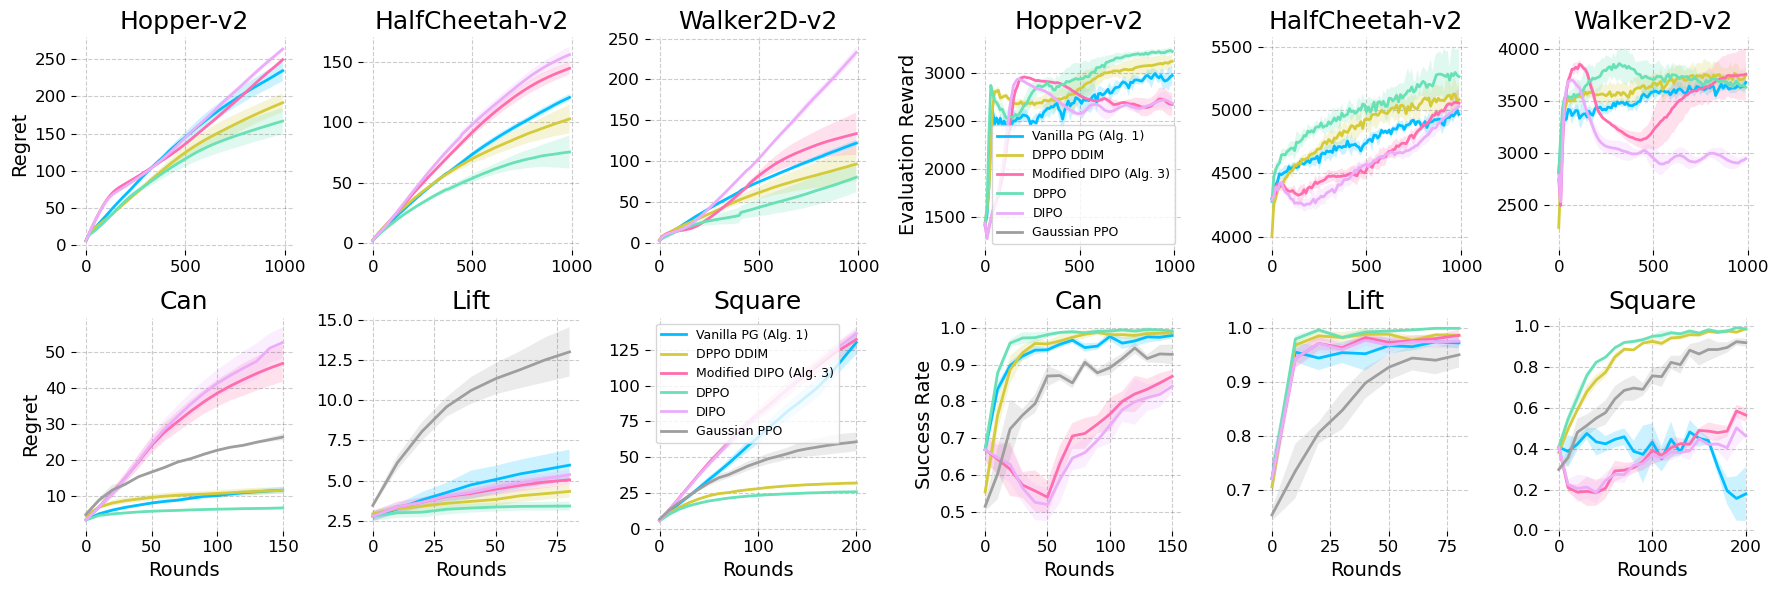
\includegraphics[width=\linewidth]{figures/ch05/imgs/combined.png}
    \caption{The six plots on the left column depict cumulative reference-return regret, defined in Appendix~\ref{app:tables}, for each algorithm on each environment. The six plots on the right column depict the evaluation reward of each algorithm on each environment, where the Gym environments are evaluated on the actual reward function and the Robomimic environments are evaluated on the success rate, as in \citet{ren2024diffusionpolicypolicyoptimization}. 95\% CI over 5 seeds.}
    \label{fig:combined}
\end{figure*}
\noindent



\section{Numerical Experiments}\label{ch05:sec:experiments}



To investigate how our theory holds up empirically, building on the work of \citet{ren2024diffusionpolicypolicyoptimization}, we provide experiments on the \{Hopper, Walker2D, HalfCheetah\} Gym \citep{brockman2016openaigym, towers2025gymnasiumstandardinterfacereinforcement} and \{Can, Square, Lift\} Robomimic \citep{robomimic2021} environments that investigate whether a representative array of diffusion policy algorithms exhibit sublinear empirical regret.
Two are the ones we base our paper on (DPPO \cite{ren2024diffusionpolicypolicyoptimization} and DIPO \cite{yang2023policyrepresentationdiffusionprobability}), and another is a PPO-trained Gaussian policy on Robomimic. 
We implement three more practical variants motivated by Algorithms~\ref{alg:dppo-vanilla-pg}--\ref{alg:dipo-bc}. The first modifies DPPO to use the vanilla policy gradient update (with a step size an order of magnitude smaller). DPPO+DDIM uses PPO with a DDIM sampler, rather than the least-squares NPG update in Algorithm~\ref{alg:dppo-reinforce}. The last modifies DIPO to use separate datasets for behavior cloning and critic estimation as described in Section \ref{sec:behavior-clone}. These are labeled Vanilla PG, DPPO DDIM, and Modified DIPO respectively. All experiments were run on two RTX 3090 GPUs, taking around a week. Hyperparameters are identical to \cite{ren2024diffusionpolicypolicyoptimization}, except for a learning rate an order of magnitude smaller for vanilla policy gradients.


The experiments are run on five seeds, $42,43,44,45,46$, in sequence from the seed used in
\citet{ren2024diffusionpolicypolicyoptimization}. We report means and 95\% confidence intervals. In line with \cite{ren2024diffusionpolicypolicyoptimization}, we employ a critic with generalized advantage estimation \citep{schulman2018gae} instead of using advantage estimates from Algorithm \ref{alg:dppo-sampler}. Further tables with CIs over seeds depicting the best value achieved by each algorithm, normalized regret statistics, and fits of the regret exponent $T^\alpha$ for each environment can be found in Appendix \ref{app:tables}.


\begin{table}[H]

    \centering
    \small
    \renewcommand{\arraystretch}{1.15}
    \begin{tabular}{|l|c|c|c|c|}
        \hline \bf Algorithm & \bf Regret & \bf Value & \bf  Sublinear & \bf Exponent \\
        \hline DPPO & 1.00 & 1.00 & 5/6 & 0.77 \\
        \hline DPPO+DDIM & 2.00 & 2.17 & 6/6 & 0.68 \\
        \hline Vanilla PG (\ref{alg:dppo-vanilla-pg}) & 3.50 & 4.50 & 5/6 & 1.03 \\
        \hline Modified DIPO (\ref{alg:dipo-bc}) & 4.17 & 3.50 & 4/6 & 0.85 \\
        \hline Gaussian PPO & 4.33 & 4.33 & 3/3 & 0.51 \\
        \hline DIPO & 5.17 & 4.67 & 4/6 & 1.25 \\
        \hline
        \end{tabular}

    \caption{Average rank across environments for plotted regret and best value. Number of environments rejecting $\alpha\ge1$ after Holm correction. Largest late-half fitted exponent across environments.}
    \label{tab:statistics}
\end{table}
\noindent


\paragraph{Diffusion policies can exhibit sublinear empirical regret.}
Figure~\ref{fig:combined} and Table~\ref{tab:statistics} show that most diffusion-policy methods exhibit sublinear empirical regret on most environments. The per-seed tests in Appendix~\ref{app:tables} reject an exponent of at least one in $15$ of the $18$ cells for Vanilla PG, DPPO+DDIM, and Modified DIPO. Not every method is sublinear on
every environment. The modified DIPO variant improves over DIPO on most tasks by decoupling critic estimation
from behavior cloning.


\paragraph{Policy optimization versus critic cloning.}
The results should not be read as contradicting Theorem \ref{thm:dipo-bc-regret}. The bound contains score-matching and sampler-approximation terms. When the score
model is learned online from scratch, as it is within the numerical experiments, these terms can dominate early training. Policy optimization
has a weaker asymptotic rate in our theory, but it does not need to repeatedly score-match a moving
critic-induced greedy policy. This may help explain why DPPO-style methods can outperform DIPO-style
methods in our experiments, even though Theorem \ref{thm:dipo-bc-regret} has better dependence in $T$ when the cloning and sampler errors are controlled. Table~\ref{tab:actor-loss} examines the empirical denoising losses, whose association with regret is inconclusive.

% The experiments are run on five seeds in sequence from seed 42, the same seed employed in the source code from \citet{ren2024diffusionpolicypolicyoptimization}. In line with them, we employ a critic with generalized advantage estimation \citep{schulman2018gae} instead of using advantage estimates from Algorithm \ref{alg:dppo-sampler}. 

% We plot the results in Figure \ref{fig:combined}, with relevant statistics in Table \ref{tab:statistics}.
% Further tables depicting the best value achieved by each algorithm, normalized regret statistics, and subjective assessments of whether each algorithm achieved sublinear regret on each environment can be found in Appendix \ref{app:tables}.



% \paragraph{Diffusion policies achieve sublinear regret.} Figure~\ref{fig:combined} and Table~\ref{tab:statistics} show that most algorithms achieve sublinear regret on most environments. Only DIPO, which suffers from the problems outlined in Section~\ref{sec:behavior-clone}, did not. 
% Vanilla PG (Alg. 1) is a surprisingly competitive baseline, achieving sublinear regret on all environments but Square.



% \vspace{-1.5ex}
% \paragraph{Policy optimization outperforms behavior cloning.} Although modified DIPO (Alg.~\ref{alg:dipo-bc}) improves over DIPO on most environments except marginally on Square as our theory suggests, both behavior cloning algorithms are largely dominated by the policy gradient algorithms. Still, the behavior cloning algorithms remain competitive on most tasks except for Can and Square.


\paragraph{The advantage of diffusion policies.} Gaussian PPO exhibits sublinear empirical regret on Robomimic, but DPPO and DPPO+DDIM attain higher reported values and lower normalized regret (Tables~\ref{tab:value}--\ref{tab:normalized-regret}). Their actor parameter counts are similar, with the diffusion actors using 4.27--7.10\% more parameters (Table~\ref{tab:actor-counts}). The diffusion actors also start from higher returns, so these comparisons do not isolate the effect of the policy class at matched initialization.



\paragraph{Practical takeaways.} Our theory and experiments therefore suggest practical guidance for practitioners. We suggest that users employ policy optimization as a robust option when accurate score estimates are unavailable, and to employ behavior cloning when a good score model or a warm start allows the actor to track the changing critic, as then the improved scaling in $T$ may become meaningful.


\section{Conclusion, Limitations and Future Work}


% We analyze two representative classes of algorithms for learning diffusion policies. The first includes mini-batch policy gradient methods (PG and NPG), which achieve $T^{3/4}$ regret with a high-quality reset distribution. Notably, NPG combined with DDIM can be effective with a poor reset distribution if an offline dataset is available. 
% The second involves learning a critic while imitating the induced greedy policy, attaining $\sqrt{T}$ regret, assuming accurate score estimates. When an offline dataset is accessible, optimism can be omitted, resulting in a computationally efficient algorithm.
% More discussion can be found in Appendix~\ref{app:remarks}.

% Our results provide regret guarantees for representative diffusion-policy learning paradigms rather than a complete theory of all diffusion policy RL. The policy gradient results clarify the role of coverage: vanilla PG pays a density-ratio term, while DDIM NPG replaces this with feature-covariance and compatible-approximation conditions. The cleanest NPG analysis is for DDIM; extending the same argument to DDPM requires handling errors-in-features from the stochastic denoising path. The critic-cloning result shows how optimism can remove reset coverage, with the remaining cost appearing through behavior-cloning/score-matching accuracy. Hybrid RL similarly replaces reset coverage or optimism with offline Bellman-error coverage. As such, it would be interesting to characterize exactly where diffusion policies outperform e.g. Gaussian policies other than the obvious case where the diffusion policy class is realizable but the simpler class is not.

We provide sublinear regret guarantees for two representative diffusion-policy learning paradigms.
For policy optimization, vanilla PG and DDIM NPG achieve $T^{3/4}$ regret under reset or mixing access and coverage, up to approximation and comparator errors, with
NPG removing the explicit density-ratio dependence at the cost of score-feature and covariance conditions. Hybrid NPG preserves this exponent with importance-weighted Monte Carlo labels from logged behavior trajectories under finite weighted-return moments and improved mixture conditioning.
For critic cloning, an optimistic critic plus diffusion behavior cloning gives a critic contribution of $O(H^2\sqrt{\beta T\mathsf{SEC}(\gF,\Pi,T)})$ plus cumulative actor and sampler error, and offline Bellman-error coverage can replace optimism in the hybrid setting.


Extending the NPG argument to DDPM requires handling errors-in-features from the stochastic denoising path.
Appendix~\ref{app:representation} gives a finite-sample imitation separation from flat Gaussian mixtures for structured product-mixture targets. Whether diffusion policies improve RL regret or sample efficiency over Gaussian policies and flat Gaussian mixtures under the same objective and data access remains open.
More discussion can be found in Appendix~\ref{app:remarks}.

% Much future work remains. We believe that matching the score estimate to the critic's action gradient as in \citet{psenka2024learningdiffusionmodelpolicy} may provide provable guarantees in the specific case where Q-score matching can be viewed as matching the softmax policy induced by the current critic. In this case, one can combine our analysis and that of \citet{tan2025actorcriticsachieveoptimalsample} to do so. However, this equivalence to softmax policy score-matching only holds in very limited circumstances. An alternative is to use an analogous notion to that of compatible function approximation \citep{sutton1999policygradient}, but with gradients with respect to actions, to view this as score-matching with respect to some policy induced by the current critic. Other than that, it is unclear to us what provable guarantees, if any, can be shown in general.
Our work leaves several compelling directions open. Matching  the score estimate with the critic’s action gradient, as in \cite{psenka2024learningdiffusionmodelpolicy}, may yield provable guarantees in settings where Q-score matching amounts to matching the softmax policy induced by the current critic. In such cases, it may be possible to integrate our analysis with that of \cite{tan2025actorcriticsachieveoptimalsample} to establish theoretical guarantees. 
An alternative option involves extending the idea of compatible function approximation \citep{sutton1999policygradient} using action gradients to reinterpret score-matching with respect to some policy derived from the current critic. 

% 